\documentclass[11pt]{article}
\usepackage[margin=1in]{geometry}
\usepackage{amsmath}
\usepackage{booktabs}
\usepackage{graphicx}
\usepackage{float}
\usepackage{caption}
\usepackage[hidelinks]{hyperref}
\usepackage{tikz}
\usetikzlibrary{positioning,fit,arrows.meta,calc}

\newcommand{\invlogit}{\operatorname{logit}^{-1}}
\newcommand{\code}[1]{\texttt{#1}}

\graphicspath{{Plots_C/Convergence_Plots_C/}}

\title{Convergence Simulations Model C}
\author{Vera Schroeder}
\date{October 2026}

\begin{document}

\maketitle


\section{Model Structure}

Model C is Model B (hierarchical over sessions) with the distractor entering the
psychometric function as a covariate. Instead of fitting unimanual and bimanual
trials as separate groups, it adds a term $\beta_2 d$ for the distractor
amplitude $d$, so the groups are the two hands.

\subsection{Data and indexing}
The data are $N$ binary trials. Trial $i$ has
\begin{itemize}
  \item a response $y_i \in \{0,1\}$, the monkey's categorization of the stimulus as ``low'' (0) or ``high'' (1);
  \item a standardized stimulus amplitude $x_i$. As in Models A and B, the raw
        amplitudes are centered and scaled by the mean and standard deviation of the
        distinct amplitude levels;
  \item a distractor covariate $d_i$: the distractor amplitude divided by the same
        standard deviation (14.63) but not centered, so that $d_i = 0$ on unimanual
        trials (no distractor). On bimanual trials $d_i$ ranges from 0.41
        (amplitude 6) to 2.19 (amplitude 32). The covariate row is
        $(1, x_i, d_i)$;
  \item a hand $j[i] \in \{\text{left}, \text{right}\}$;
  \item a session $s[i] \in \{1,\dots,S\}$; the real data have $S = 42$.
\end{itemize}
Every session uses a single distractor amplitude on its bimanual trials, so within a
session $d_i$ only switches between 0 and that session's value $d_s$. The real
sessions use 11 different amplitudes, most often 32 (13 sessions), 6 (8 sessions),
24 (7 sessions) and 12 (6 sessions).

\subsection{Likelihood}

Each response is Bernoulli,
\[
  y_i \sim \text{Bernoulli}(\psi_i), \qquad
  \psi_i = \psi\big(x_i, d_i;\ \theta_{j[i],s[i]}\big),
\]
with the psychometric function
\[
  \psi(x, d;\theta) = \gamma_h + (1 - \gamma_h - \gamma_l)\,\invlogit(\beta_0 + \beta_1 x + \beta_2 d),
  \qquad \theta = (\beta_0, \beta_1, \beta_2, \gamma_h, \gamma_l).
\]
As in Model B, $\gamma_h$ is the probability of responding ``high'' at very low
amplitudes and $\gamma_l$ the probability of responding ``low'' at very high
amplitudes. $\beta_2$ shifts the curve on bimanual trials in proportion to the
distractor amplitude: a positive $\beta_2$ makes ``high'' responses more likely,
moving the PSE to lower amplitudes. The lapse rates are shared by the unimanual and
bimanual trials of a hand and session. In the code $\psi_i$ is clipped to
$[10^{-8},\,1-10^{-8}]$ before entering the Bernoulli likelihood, for numerical
stability.

\subsection{Session-level}

For each hand $j$ and session $s$, the five parameters are drawn independently
from hand-specific distributions:
\begin{align*}
  \beta_{k,js} &\sim \mathcal{N}\big(\mu_{\beta_k,j},\ \sigma_{\beta_k,j}\big), \qquad k = 0, 1, 2, \\
  \gamma_{h,js} &= 0.25\, w_{h,js}, \qquad
      w_{h,js} \sim \text{LogitNormal}\big(\mu_{\gamma_h,j},\ \sigma_{\gamma_h,j}\big), \\
  \gamma_{l,js} &= 0.25\, w_{l,js}, \qquad
      w_{l,js} \sim \text{LogitNormal}\big(\mu_{\gamma_l,j},\ \sigma_{\gamma_l,j}\big).
\end{align*}
The two hands are independent of each other (no pooling across hands).

\subsection{Hand-level Hyperpriors}

Each hand has 10 hyperparameters. Those of $\beta_0$, $\beta_1$ and the lapse rates
have the same priors as in Model B:
\begin{align*}
  \mu_{\beta_0,j} &\sim \mathcal{N}(0,\ 2), &
  \sigma_{\beta_0,j} &\sim \text{HalfNormal}(2), \\
  \mu_{\beta_1,j} &\sim \text{LogNormal}(\log 4,\ 0.5), &
  \sigma_{\beta_1,j} &\sim \text{Exponential}(\lambda = 1), \\
  \mu_{\beta_2,j} &\sim \mathcal{N}(0,\ 1), &
  \sigma_{\beta_2,j} &\sim \text{HalfNormal}(1), \\
  \mu_{\gamma_h,j},\ \mu_{\gamma_l,j} &\sim \mathcal{N}(-3,\ 1.5), &
  \sigma_{\gamma_h,j},\ \sigma_{\gamma_l,j} &\sim \text{HalfNormal}(0.5).
\end{align*}
All hyperparameters are independent. The Model B report explains the priors shared
with Model B. The priors of $\beta_2$ were chosen from what the parameter means, not
from fits to the real data:
\begin{itemize}
  \item $\mu_{\beta_2}$: centered at 0 because the distractor could push responses
        either way. With $d$ at most 2.19, the typical shift $\mu_{\beta_2} d$ at the
        largest distractor lies within $\pm 4.3$ logits with 95\% prior probability,
        the same scale as the prior on $\mu_{\beta_0}$.
  \item $\sigma_{\beta_2}$: median 0.67, 95\% point 1.96, allowing sessions to differ
        in their distractor effect by about as much as the hand-level effect itself.
\end{itemize}

\subsection{Graphical Model}

\begin{center}
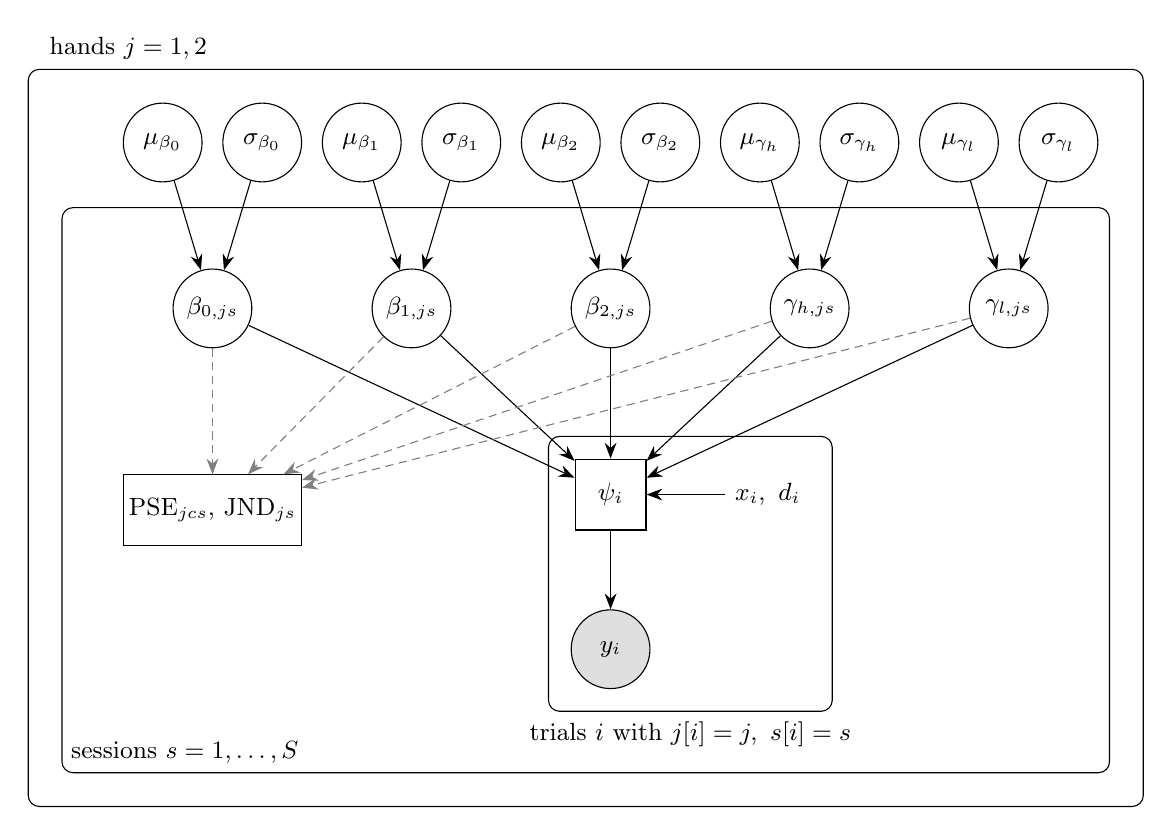
\begin{tikzpicture}[
    node distance=1.1cm and 0.25cm,
    latent/.style={circle, draw, minimum size=10mm, inner sep=0pt, font=\small},
    obs/.style={latent, fill=gray!25},
    det/.style={rectangle, draw, minimum size=9mm, inner sep=2pt, font=\small},
    const/.style={font=\small},
    arr/.style={-{Stealth[length=2mm]}},
    plate/.style={draw, rounded corners, inner sep=8pt}
  ]
  % hyperparameters
  \node[latent] (mub0) {$\mu_{\beta_0}$};
  \node[latent, right=of mub0] (sb0) {$\sigma_{\beta_0}$};
  \node[latent, right=of sb0] (mub1) {$\mu_{\beta_1}$};
  \node[latent, right=of mub1] (sb1) {$\sigma_{\beta_1}$};
  \node[latent, right=of sb1] (mub2) {$\mu_{\beta_2}$};
  \node[latent, right=of mub2] (sb2) {$\sigma_{\beta_2}$};
  \node[latent, right=of sb2] (mugh) {$\mu_{\gamma_h}$};
  \node[latent, right=of mugh] (sgh) {$\sigma_{\gamma_h}$};
  \node[latent, right=of sgh] (mugl) {$\mu_{\gamma_l}$};
  \node[latent, right=of mugl] (sgl) {$\sigma_{\gamma_l}$};

  % session-level parameters
  \node[latent, below=1.6cm of $(mub0)!0.5!(sb0)$] (b0) {$\beta_{0,js}$};
  \node[latent, below=1.6cm of $(mub1)!0.5!(sb1)$] (b1) {$\beta_{1,js}$};
  \node[latent, below=1.6cm of $(mub2)!0.5!(sb2)$] (b2) {$\beta_{2,js}$};
  \node[latent, below=1.6cm of $(mugh)!0.5!(sgh)$] (gh) {$\gamma_{h,js}$};
  \node[latent, below=1.6cm of $(mugl)!0.5!(sgl)$] (gl) {$\gamma_{l,js}$};

  % derived
  \node[det, below=1.6cm of b0] (pse) {PSE$_{jcs}$, JND$_{js}$};

  % trial level
  \node[det, below=1.4cm of b2] (psi) {$\psi_i$};
  \node[obs, below=1.0cm of psi] (y) {$y_i$};
  \node[const, right=1.0cm of psi] (x) {$x_i,\ d_i$};

  \foreach \h/\p in {mub0/b0, sb0/b0, mub1/b1, sb1/b1, mub2/b2, sb2/b2, mugh/gh, sgh/gh, mugl/gl, sgl/gl}
    \draw[arr] (\h) -- (\p);
  \foreach \p in {b0, b1, b2, gh, gl}
    \draw[arr] (\p) -- (psi);
  \foreach \p in {b0, b1, b2, gh, gl}
    \draw[arr, densely dashed, gray] (\p) -- (pse);
  \draw[arr] (x) -- (psi);
  \draw[arr] (psi) -- (y);

  % plates
  \node[plate, fit=(x)(psi)(y), label={[font=\small]below:{trials $i$ with $j[i]=j,\ s[i]=s$}}] (ptrial) {};
  \node[plate, fit=(b0)(gl)(pse)(ptrial), inner sep=22pt,
        label={[font=\small, anchor=south west]south west:{sessions $s = 1,\dots,S$}}] (psess) {};
  \node[plate, fit=(mub0)(sgl)(psess), inner sep=12pt,
        label={[font=\small]above left:{hands $j = 1, 2$}}] {};
\end{tikzpicture}
\end{center}

\noindent
Circles are random variables (shaded: observed), rectangles are deterministic
functions, and $x_i, d_i$ are fixed covariates. Dashed arrows lead to derived
quantities that do not feed back into the likelihood.

\subsection{Derived Quantities: PSE and JND}

The PSE now depends on the distractor. For each hand and session it is recorded for
both conditions $c$: unimanual ($d = 0$) and bimanual ($d = d_s$, the session's
distractor). Solving $\psi = \tfrac12$ for $x$ gives
\[
  \text{PSE}_{c} = \frac{1}{\beta_1}\left[-\big(\beta_0 + \beta_2 d\big) + \log\frac{1-2\gamma_h}{1-2\gamma_l}\right],
  \qquad d = 0 \text{ (uni)},\ d_s \text{ (bi)}.
\]
The JND does not depend on the distractor, since $\beta_2 d$ only shifts the curve:
\[
  \text{JND} = \frac{1}{2\beta_1}\,\log\frac{(3-4\gamma_h)(3-4\gamma_l)}{(1-4\gamma_h)(1-4\gamma_l)} .
\]
Both are in units of the standardized stimulus.

\subsection{Implementation}

As in Model B, the distributions are written as deterministic transforms of
standard random variables (non-centered parameterizations). Unlike Model B, the
HalfNormal sds $\sigma_{\beta_0}$, $\sigma_{\beta_2}$, $\sigma_{\gamma_h}$ and
$\sigma_{\gamma_l}$ are scaled HalfNormal(1) variables rather than absolute values of
standard normals: with the absolute value the sign is not identified, chains settle
on opposite signs, and the sampler diagnostics report a failure that does not affect
the model. The two forms define the same prior.

\section{Synthetic Data Generation}

The synthetic data follow Model C with true hyperparameters derived from Model B's
fit to the real data (posterior means in \code{Results\_B.pkl}), so that they
resemble the real data. These values only generate data; the priors do not use them.
Model B has no $\beta_2$ and fits unimanual and bimanual trials separately, so for
each hand (\code{SynthData\_C.py}):
\begin{itemize}
  \item $\mu_{\beta_0}, \sigma_{\beta_0}$: Model B's unimanual hyperparameters
        ($\beta_0$ at $d = 0$);
  \item $\mu_{\beta_1}, \sigma_{\beta_1}$: the average of Model B's unimanual and
        bimanual hyperparameters;
  \item $\mu_{\beta_2}$: the slope through the origin of each session's bimanual shift
        in $\beta_0$ (bimanual minus unimanual posterior mean) on that session's
        $d_s$, which is what $\beta_2 d$ describes in Model C;
  \item $\sigma_{\beta_2}$: the sd across sessions of that shift divided by $d_s$;
  \item $\mu_{\gamma_h}, \mu_{\gamma_l}$: the logit of 4 times the mean lapse rate over
        all unimanual and bimanual session estimates, since Model C shares lapse rates
        between them;
  \item $\sigma_{\gamma_h}, \sigma_{\gamma_l}$: the average of Model B's unimanual and
        bimanual hyperparameters.
\end{itemize}

\begin{table}[H]
\centering
\caption{True hyperparameters. Lapse-rate hyperparameters are on the logit scale;
the typical lapse rate is $0.25\,\invlogit(\mu_\gamma)$.}
\label{tab:true}
\begin{tabular}{lcc}
\toprule
 & left & right \\
\midrule
$\mu_{\beta_0}$ / $\sigma_{\beta_0}$ & $-1.487$ / 0.763 & $-1.056$ / 1.011 \\
$\mu_{\beta_1}$ / $\sigma_{\beta_1}$ & 4.644 / 0.776 & 4.460 / 0.394 \\
$\mu_{\beta_2}$ / $\sigma_{\beta_2}$ & 0.933 / 0.622 & 1.129 / 0.831 \\
$\mu_{\gamma_h}$ / $\sigma_{\gamma_h}$ & $-2.802$ / 0.475 & $-2.414$ / 0.366 \\
$\mu_{\gamma_l}$ / $\sigma_{\gamma_l}$ & $-3.197$ / 0.383 & $-3.204$ / 0.406 \\
typical $\gamma_h$ / $\gamma_l$ & 0.0143 / 0.0098 & 0.0205 / 0.0098 \\
\bottomrule
\end{tabular}
\end{table}

Unlike the earlier hand-picked values for Model B's study, the between-session sds of
the slope are substantial (0.78 and 0.39), and those of the distractor coefficient
(0.62 and 0.83) are close to those of $\beta_0$ (0.76 and 1.01).

As in Model B's study, the model was fit to 10 dataset conditions in two sweeps, each
run twice with new data:
\begin{itemize}
  \item the sessions sweep varies the number of sessions (5, 10, 20, 40 and 80, each
        with 308 trials), mainly testing the hyperparameters;
  \item the trials sweep varies trials per session (20, 40, 80, 160 and 320, with 42
        sessions), mainly testing the session-level parameters.
\end{itemize}
Every replicate draws new session-level parameters from the true hyperparameters.
Each simulated session gets one distractor amplitude, drawn from the real sessions'
amplitudes, and its trials cycle through the four cells hand $\times$
(unimanual, bimanual), with each stimulus resampled from that cell's stimuli in the
real design. Within a replicate the datasets of a sweep are nested (the first $n$
sessions, or the first $t$ trials of every session). The real data have 42 sessions
with about 308 trials each, so the 40-session and 320-trial fits are the most
representative.

\section{Model Fit Results}

Every figure and number in this report is produced by \code{Convergence\_C.py};
the cell ``Numbers for Convergence\_C\_Report.tex'' prints the numbers that the
earlier cells do not, and also runs on the saved results without refitting.
Hyperparameter entries are averaged over the two replicates; session-level RMSEs and
coverages are pooled over them (84 sessions per hand in the trials sweep). Coverages
of the hyperparameters are over 4 fits per size (2 hands $\times$ 2 replicates).

\subsection{Sampling Diagnostics}
The 20 fits had 2 divergences in total, one each in a 5-session and a 10-session fit,
too few to bias the results. $\hat{R} \le 1.008$ and the bulk ESS is at least 532
for every hyperparameter, and $\hat{R} \le 1.007$ for every session-level parameter. The whole study takes about 0.7 hours.

\begin{table}[H]
\centering
\caption{Sampler diagnostics over both replicates. $\hat{R}$ and bulk ESS are
taken over the hyperparameters.}
\begin{tabular}{llccc}
\toprule
Sweep & Size & max $\hat{R}$ & min ESS & divergences \\
\midrule
sessions & 5   & 1.005 & 1467 & 1 \\
sessions & 10  & 1.004 & 1194 & 1 \\
sessions & 20  & 1.004 & 1447 & 0 \\
sessions & 40  & 1.003 & 1524 & 0 \\
sessions & 80  & 1.003 & 1309 & 0 \\
\midrule
trials & 20  & 1.007 & 598  & 0 \\
trials & 40  & 1.008 & 532  & 0 \\
trials & 80  & 1.008 & 553  & 0 \\
trials & 160 & 1.006 & 794  & 0 \\
trials & 320 & 1.005 & 847  & 0 \\
\bottomrule
\end{tabular}
\end{table}

\subsection{Hyperparameter means}

\begin{figure}[H]
\centering
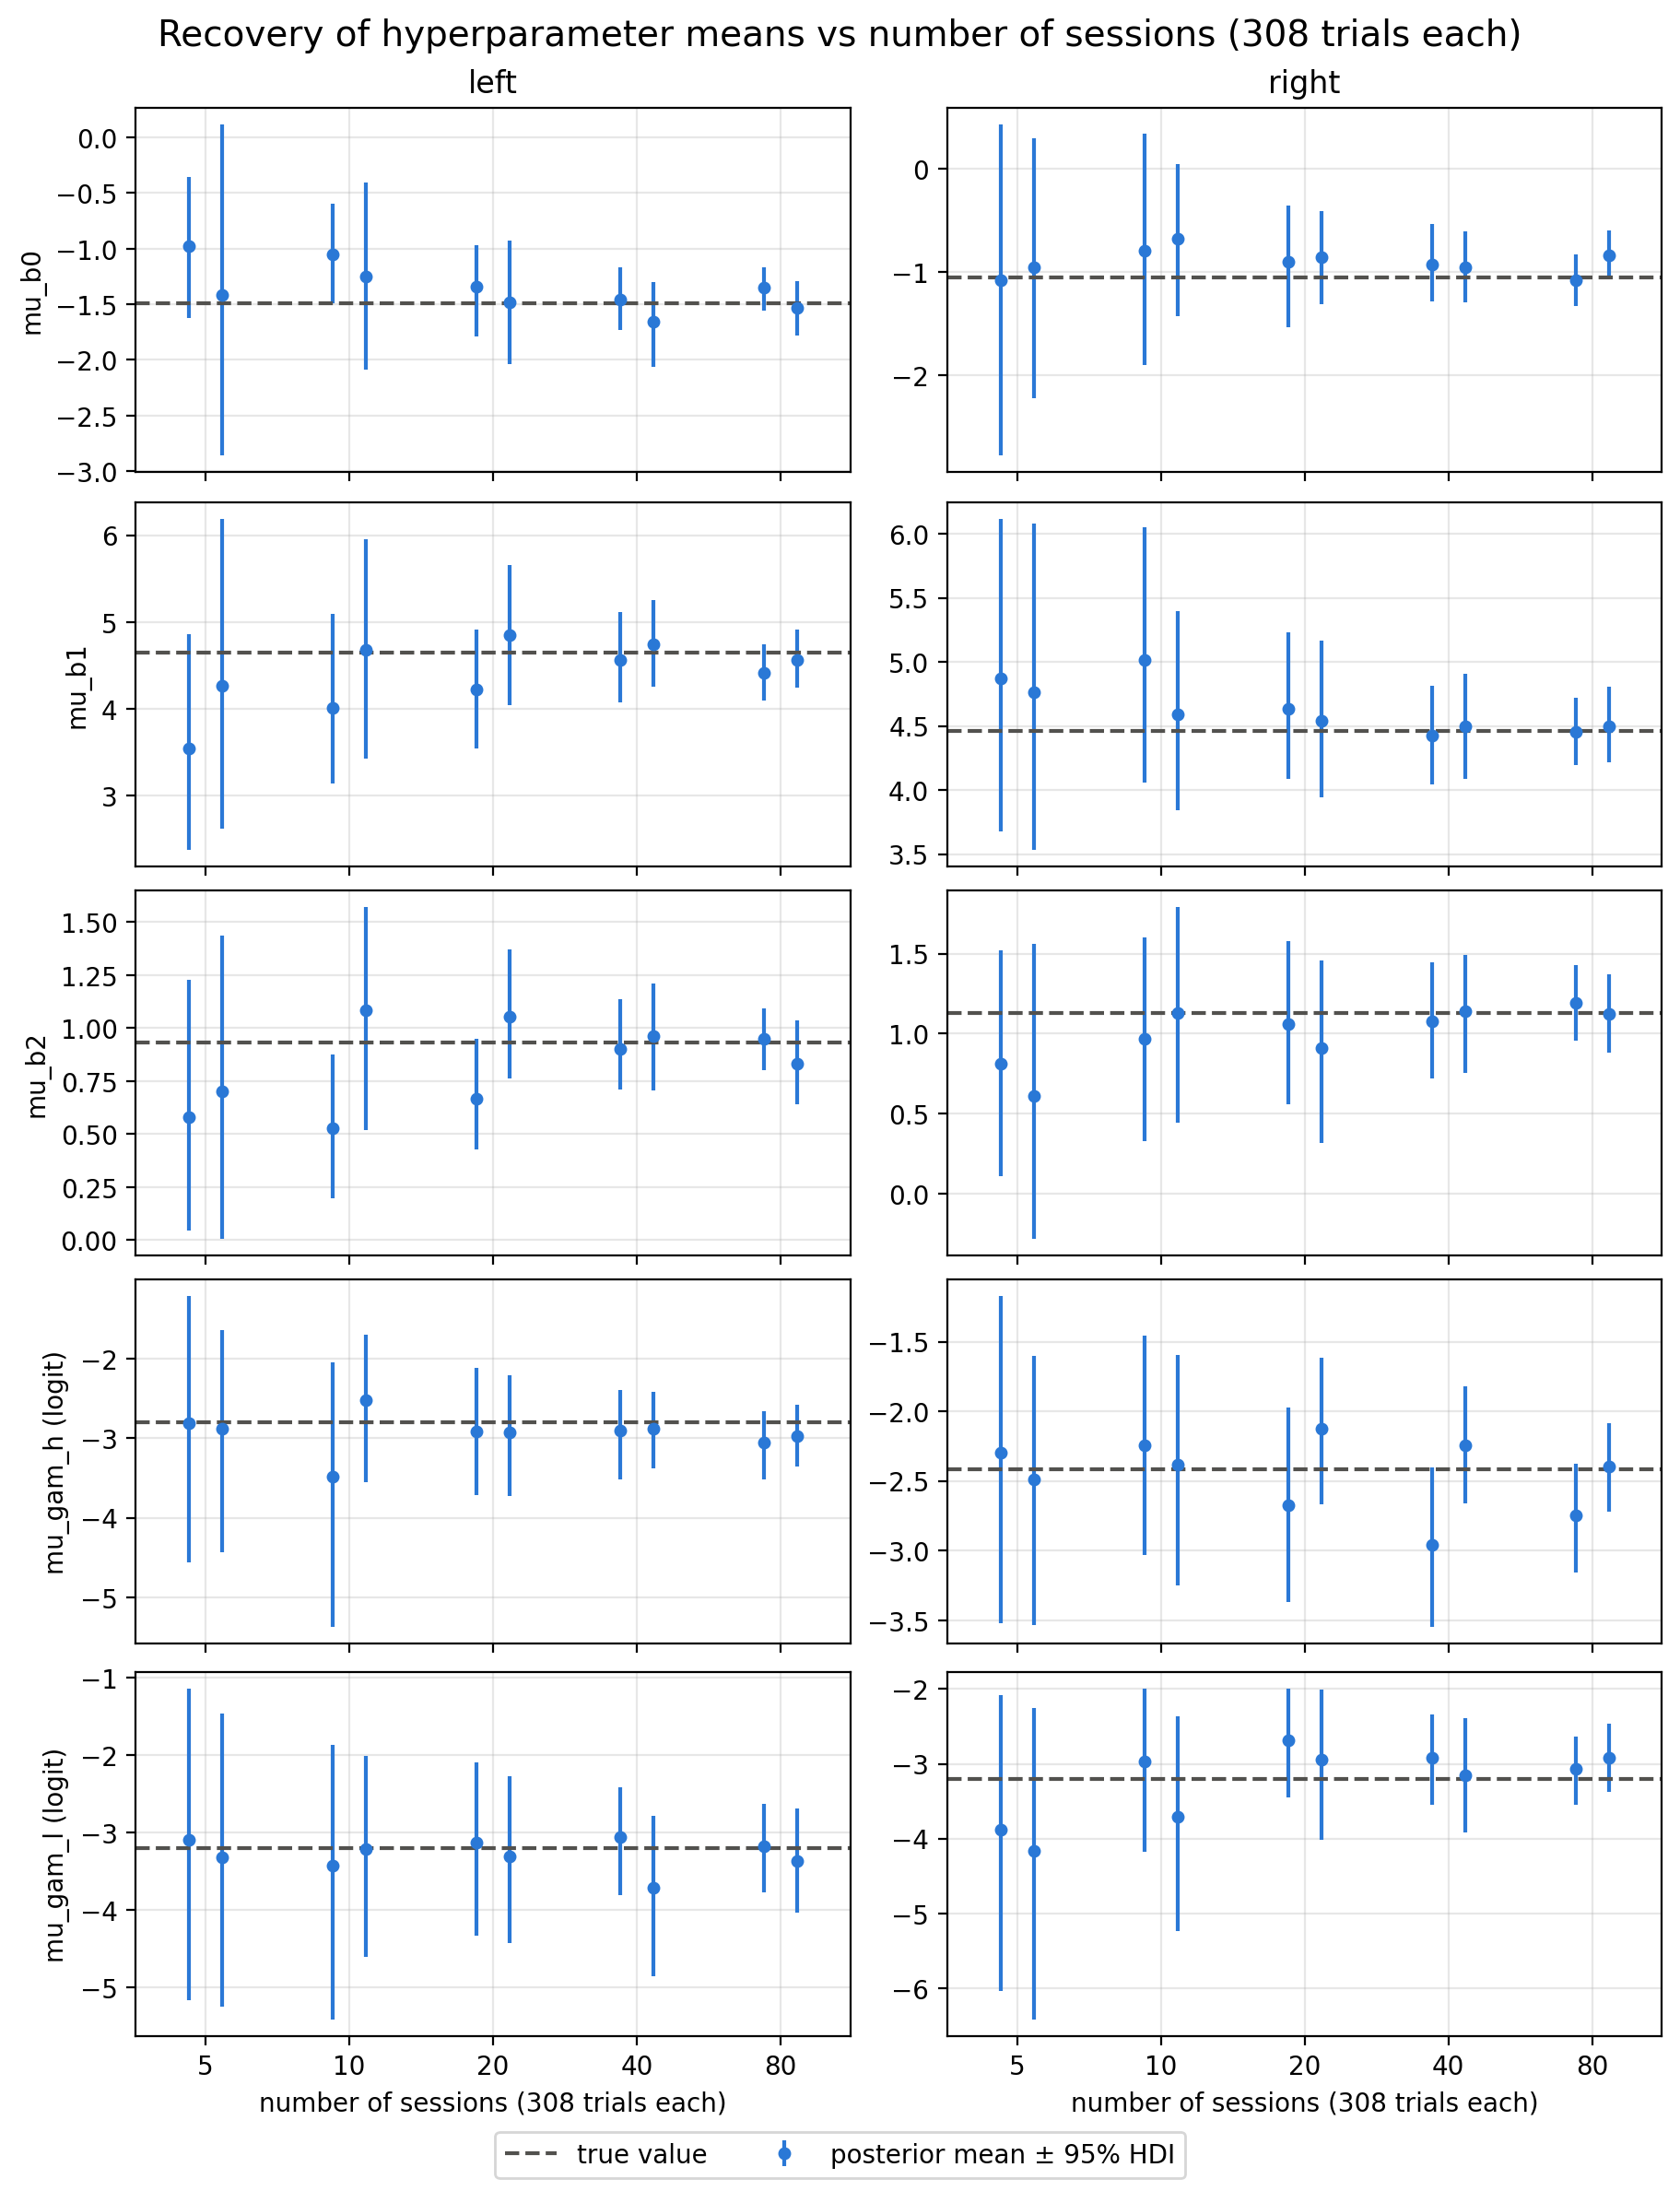
\includegraphics[width=0.9\textwidth]{hyper_means_recovery_vs_sessions.png}
\caption{Posterior mean and 95\% HDI of the hand-level means against the number of
sessions (308 trials each). The two replicates are drawn side by side; the
dashed line is the true value.}
\label{fig:means_sessions}
\end{figure}

\begin{figure}[H]
\centering
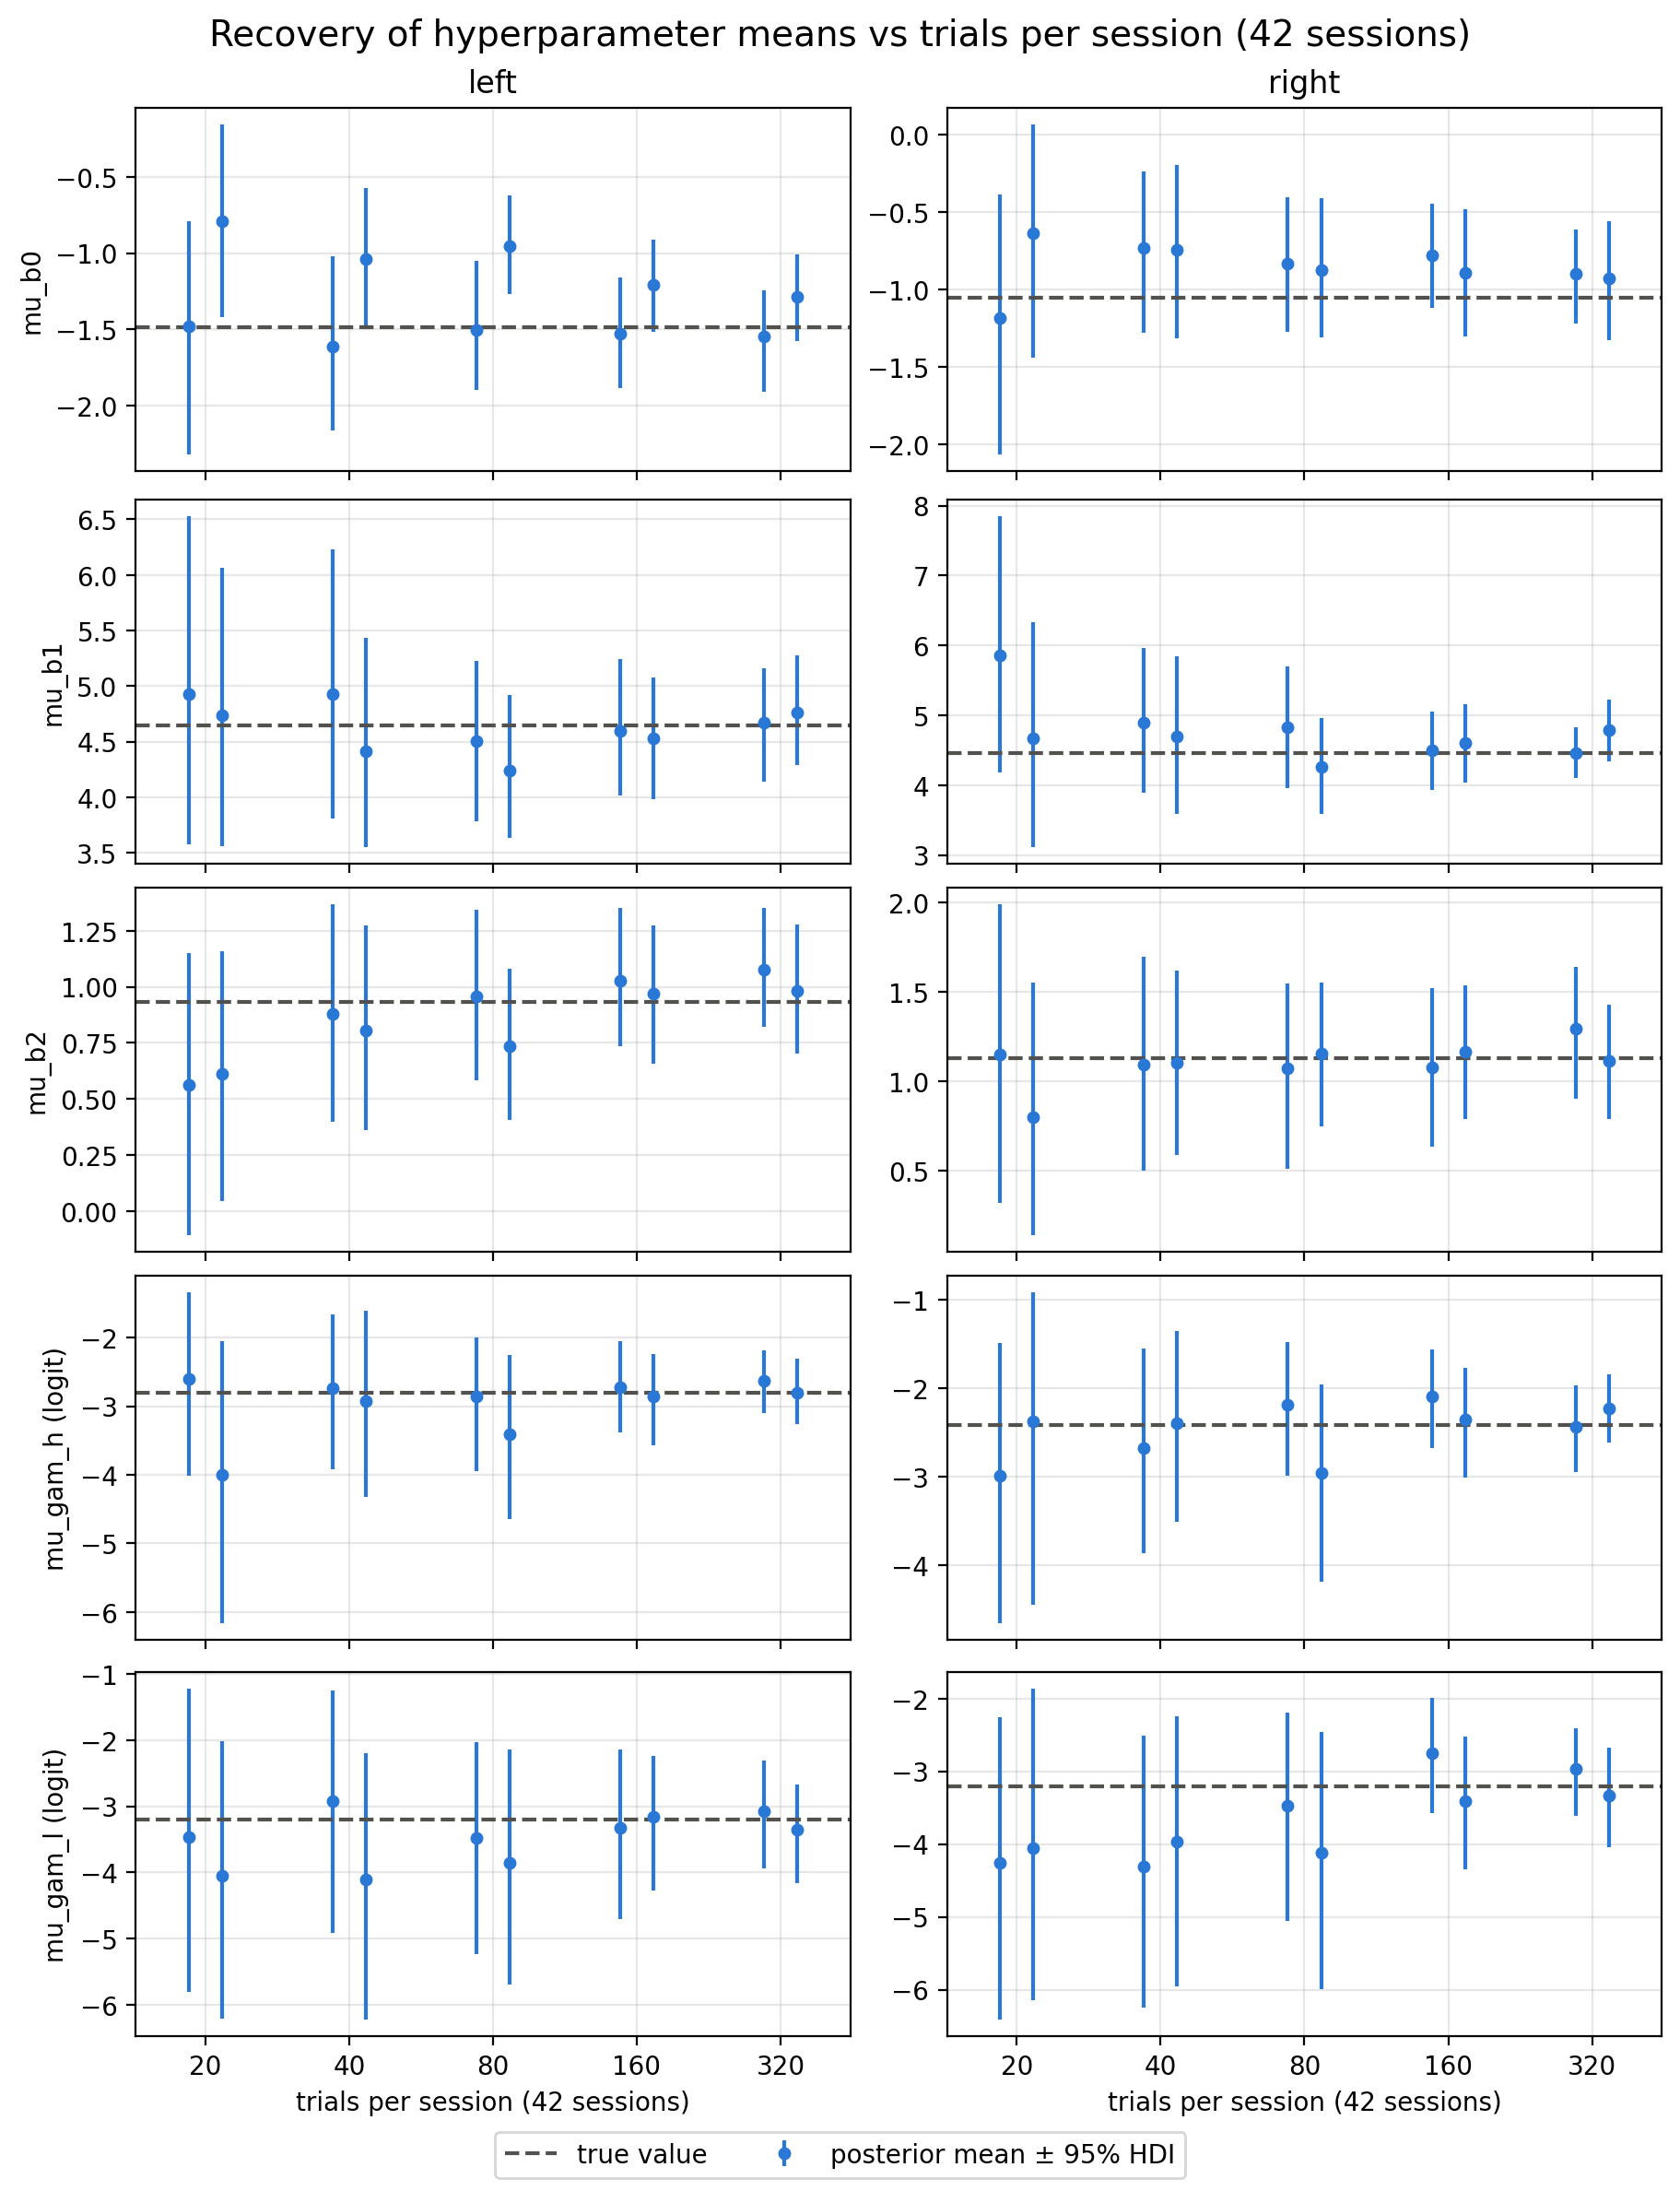
\includegraphics[width=0.9\textwidth]{hyper_means_recovery_vs_trials.png}
\caption{As Figure~\ref{fig:means_sessions}, against trials per session (42
sessions).}
\label{fig:means_trials}
\end{figure}

\begin{table}[H]
\centering
\caption{Hand-level means at 40 sessions (sessions sweep): true value and posterior
mean [95\% HDI], averaged over replicates. Lapse-rate means are on the logit scale.}
\label{tab:means40}
\begin{tabular}{lcccc}
\toprule
 & \multicolumn{2}{c}{left} & \multicolumn{2}{c}{right} \\
 & true & posterior & true & posterior \\
\midrule
$\mu_{\beta_0}$ & $-1.49$ & $-1.56$ [$-1.90$, $-1.24$] & $-1.06$ & $-0.94$ [$-1.29$, $-0.57$] \\
$\mu_{\beta_1}$ & 4.64 & 4.65 [4.16, 5.18] & 4.46 & 4.46 [4.06, 4.86] \\
$\mu_{\beta_2}$ & 0.93 & 0.93 [0.71, 1.18] & 1.13 & 1.11 [0.74, 1.47] \\
$\mu_{\gamma_h}$ & $-2.80$ & $-2.89$ [$-3.45$, $-2.41$] & $-2.41$ & $-2.60$ [$-3.10$, $-2.11$] \\
$\mu_{\gamma_l}$ & $-3.20$ & $-3.39$ [$-4.34$, $-2.60$] & $-3.20$ & $-3.04$ [$-3.73$, $-2.37$] \\
\bottomrule
\end{tabular}
\end{table}

All five hand-level means are recovered without visible bias, and in the sessions sweep
their HDIs contain the true value in every fit at 40 and 80 sessions
(Table~\ref{tab:means40}). In the trials sweep, $\mu_{\beta_0}$ misses the truth in
one of the four fits at each of 20, 40 and 80 trials. The
HDIs narrow steadily with the number of sessions; averaged over hands and replicates,
the width for $\mu_{\beta_0}$ falls from 2.49 at 5 sessions to 0.69 at 40 and 0.46 at
80.

\paragraph{Distractor effect $\mu_{\beta_2}$.} The new parameter is the
best-determined mean relative to its size: at 40 sessions the HDIs are 0.47 (left)
and 0.73 (right) wide, around true values of 0.93 and 1.13, so both exclude 0. At 5
sessions the HDI width is still 1.46 and the HDIs reach 0. In the trials
sweep, where the number of sessions is fixed at 42, the width only falls from 1.36
at 20 trials to 0.62 at 320: like the other means, $\mu_{\beta_2}$ is limited by the
number of sessions more than by trials per session.

\paragraph{Slope $\mu_{\beta_1}$.} Recovered well for both hands, in contrast with
Model B's study, where a true slope of 6 for the right hand was poorly identified. The
true slopes here, about 4.5, give a rise from $\psi = 0.25$ to 0.75 wide enough to span
several stimulus levels.

\paragraph{Lapse-rate means.} $\mu_{\gamma_h}$ and $\mu_{\gamma_l}$ are recovered,
but they are the least precise means: at 80 sessions their HDIs are still 0.71--0.82
($\mu_{\gamma_h}$) and 0.91--1.25 ($\mu_{\gamma_l}$) wide on the logit scale. Lapses
are rare and only show at the stimulus levels where the sigmoid has reached its floor
or ceiling.

\subsection{Hyperparameter standard deviations}

\begin{figure}[H]
\centering
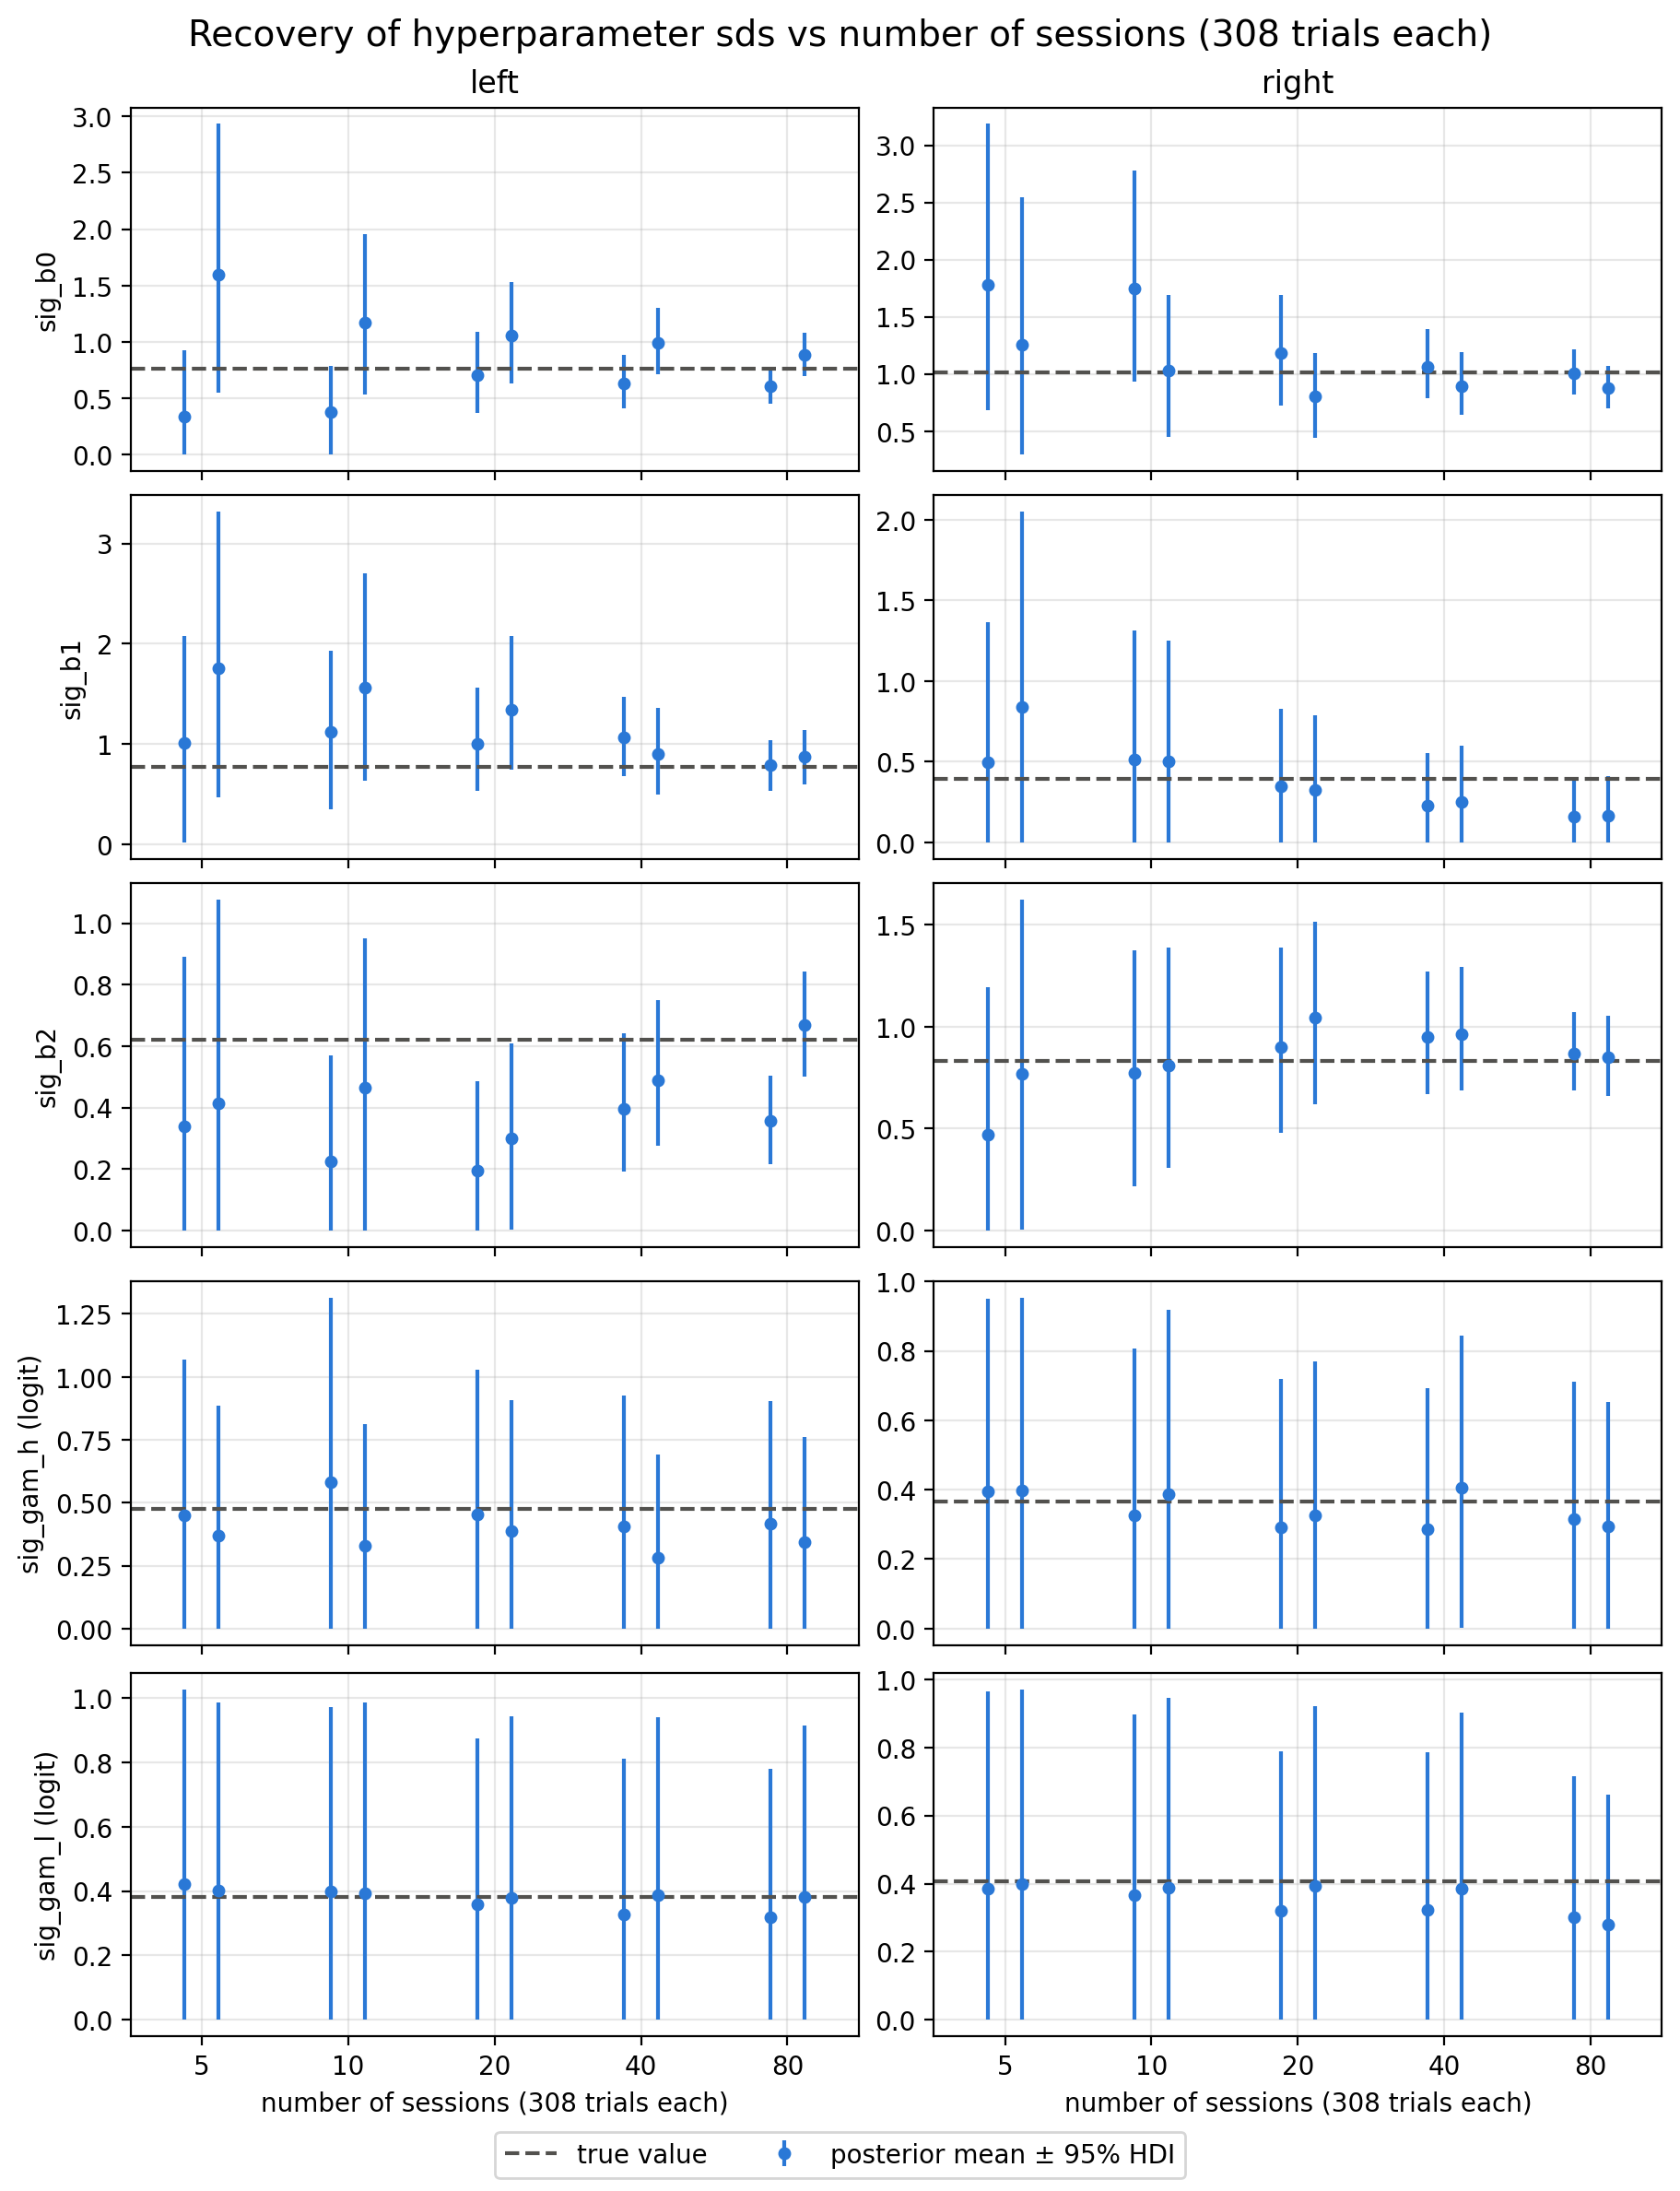
\includegraphics[width=0.9\textwidth]{hyper_sds_recovery_vs_sessions.png}
\caption{Posterior mean and 95\% HDI of the between-session standard deviations
against the number of sessions.}
\label{fig:sds_sessions}
\end{figure}

\begin{table}[H]
\centering
\caption{Between-session sds at 80 sessions (sessions sweep): true value and
posterior mean [95\% HDI], averaged over replicates, and the fraction of the two
replicates whose HDI contains the true value.}
\label{tab:sds80}
\begin{tabular}{lcccccc}
\toprule
 & \multicolumn{3}{c}{left} & \multicolumn{3}{c}{right} \\
 & true & posterior & cov. & true & posterior & cov. \\
\midrule
$\sigma_{\beta_0}$ & 0.76 & 0.74 [0.58, 0.92] & 1.0 & 1.01 & 0.94 [0.76, 1.14] & 1.0 \\
$\sigma_{\beta_1}$ & 0.78 & 0.83 [0.57, 1.09] & 1.0 & 0.39 & 0.17 [0.00, 0.40] & 0.5 \\
$\sigma_{\beta_2}$ & 0.62 & 0.51 [0.36, 0.67] & 0.5 & 0.83 & 0.86 [0.68, 1.06] & 1.0 \\
$\sigma_{\gamma_h}$ & 0.48 & 0.38 [0.00, 0.83] & 1.0 & 0.37 & 0.31 [0.00, 0.68] & 1.0 \\
$\sigma_{\gamma_l}$ & 0.38 & 0.35 [0.00, 0.85] & 1.0 & 0.41 & 0.29 [0.00, 0.69] & 1.0 \\
\bottomrule
\end{tabular}
\end{table}

\paragraph{$\sigma_{\beta_0}$, $\sigma_{\beta_1}$, $\sigma_{\beta_2}$.} The between-session
sds of the three logistic coefficients are identified: their HDIs narrow with the
number of sessions and, at 80 sessions, are 0.32--0.52 wide. Two caveats
(Table~\ref{tab:sds80}):
\begin{itemize}
  \item For the left hand, one of the two replicates misses the true $\sigma_{\beta_2}$
        at 80 sessions. In Figure~\ref{fig:sds_sessions} the
        left-hand $\sigma_{\beta_2}$ estimates lie below the truth at most sizes in
        both replicates. Whether this is a bias or the particular draws of session
        effects cannot be told from two replicates.
  \item For the right hand, $\sigma_{\beta_1}$ drifts down as sessions are added, to
        0.17 at 80 sessions against a true 0.39. Both replicates' HDIs end near the
        truth, and one of them just misses it.
        The smallest true sd of the three is the hardest to separate from zero.
\end{itemize}
In the trials sweep, $\sigma_{\beta_0}$ misses the truth in two of the four fits at 40
trials, one at 80, and none at 160 and 320.

\paragraph{Lapse-rate sds $\sigma_{\gamma_h}$, $\sigma_{\gamma_l}$.} Not identified at these
data sizes. Their HDIs always start at 0 and are still 0.68--0.85 wide at 80 sessions;
averaged over hands, the width shrinks only from about 1.0 at 5 sessions to 0.76--0.77
at 80, and the posterior means barely move. Their true
values (0.37--0.48) happen to be close to the prior median (0.34), so the 100\%
coverage says little: the posteriors largely reflect the prior.

\subsection{Session-level parameters}
\label{sec:session}

\begin{figure}[H]
\centering
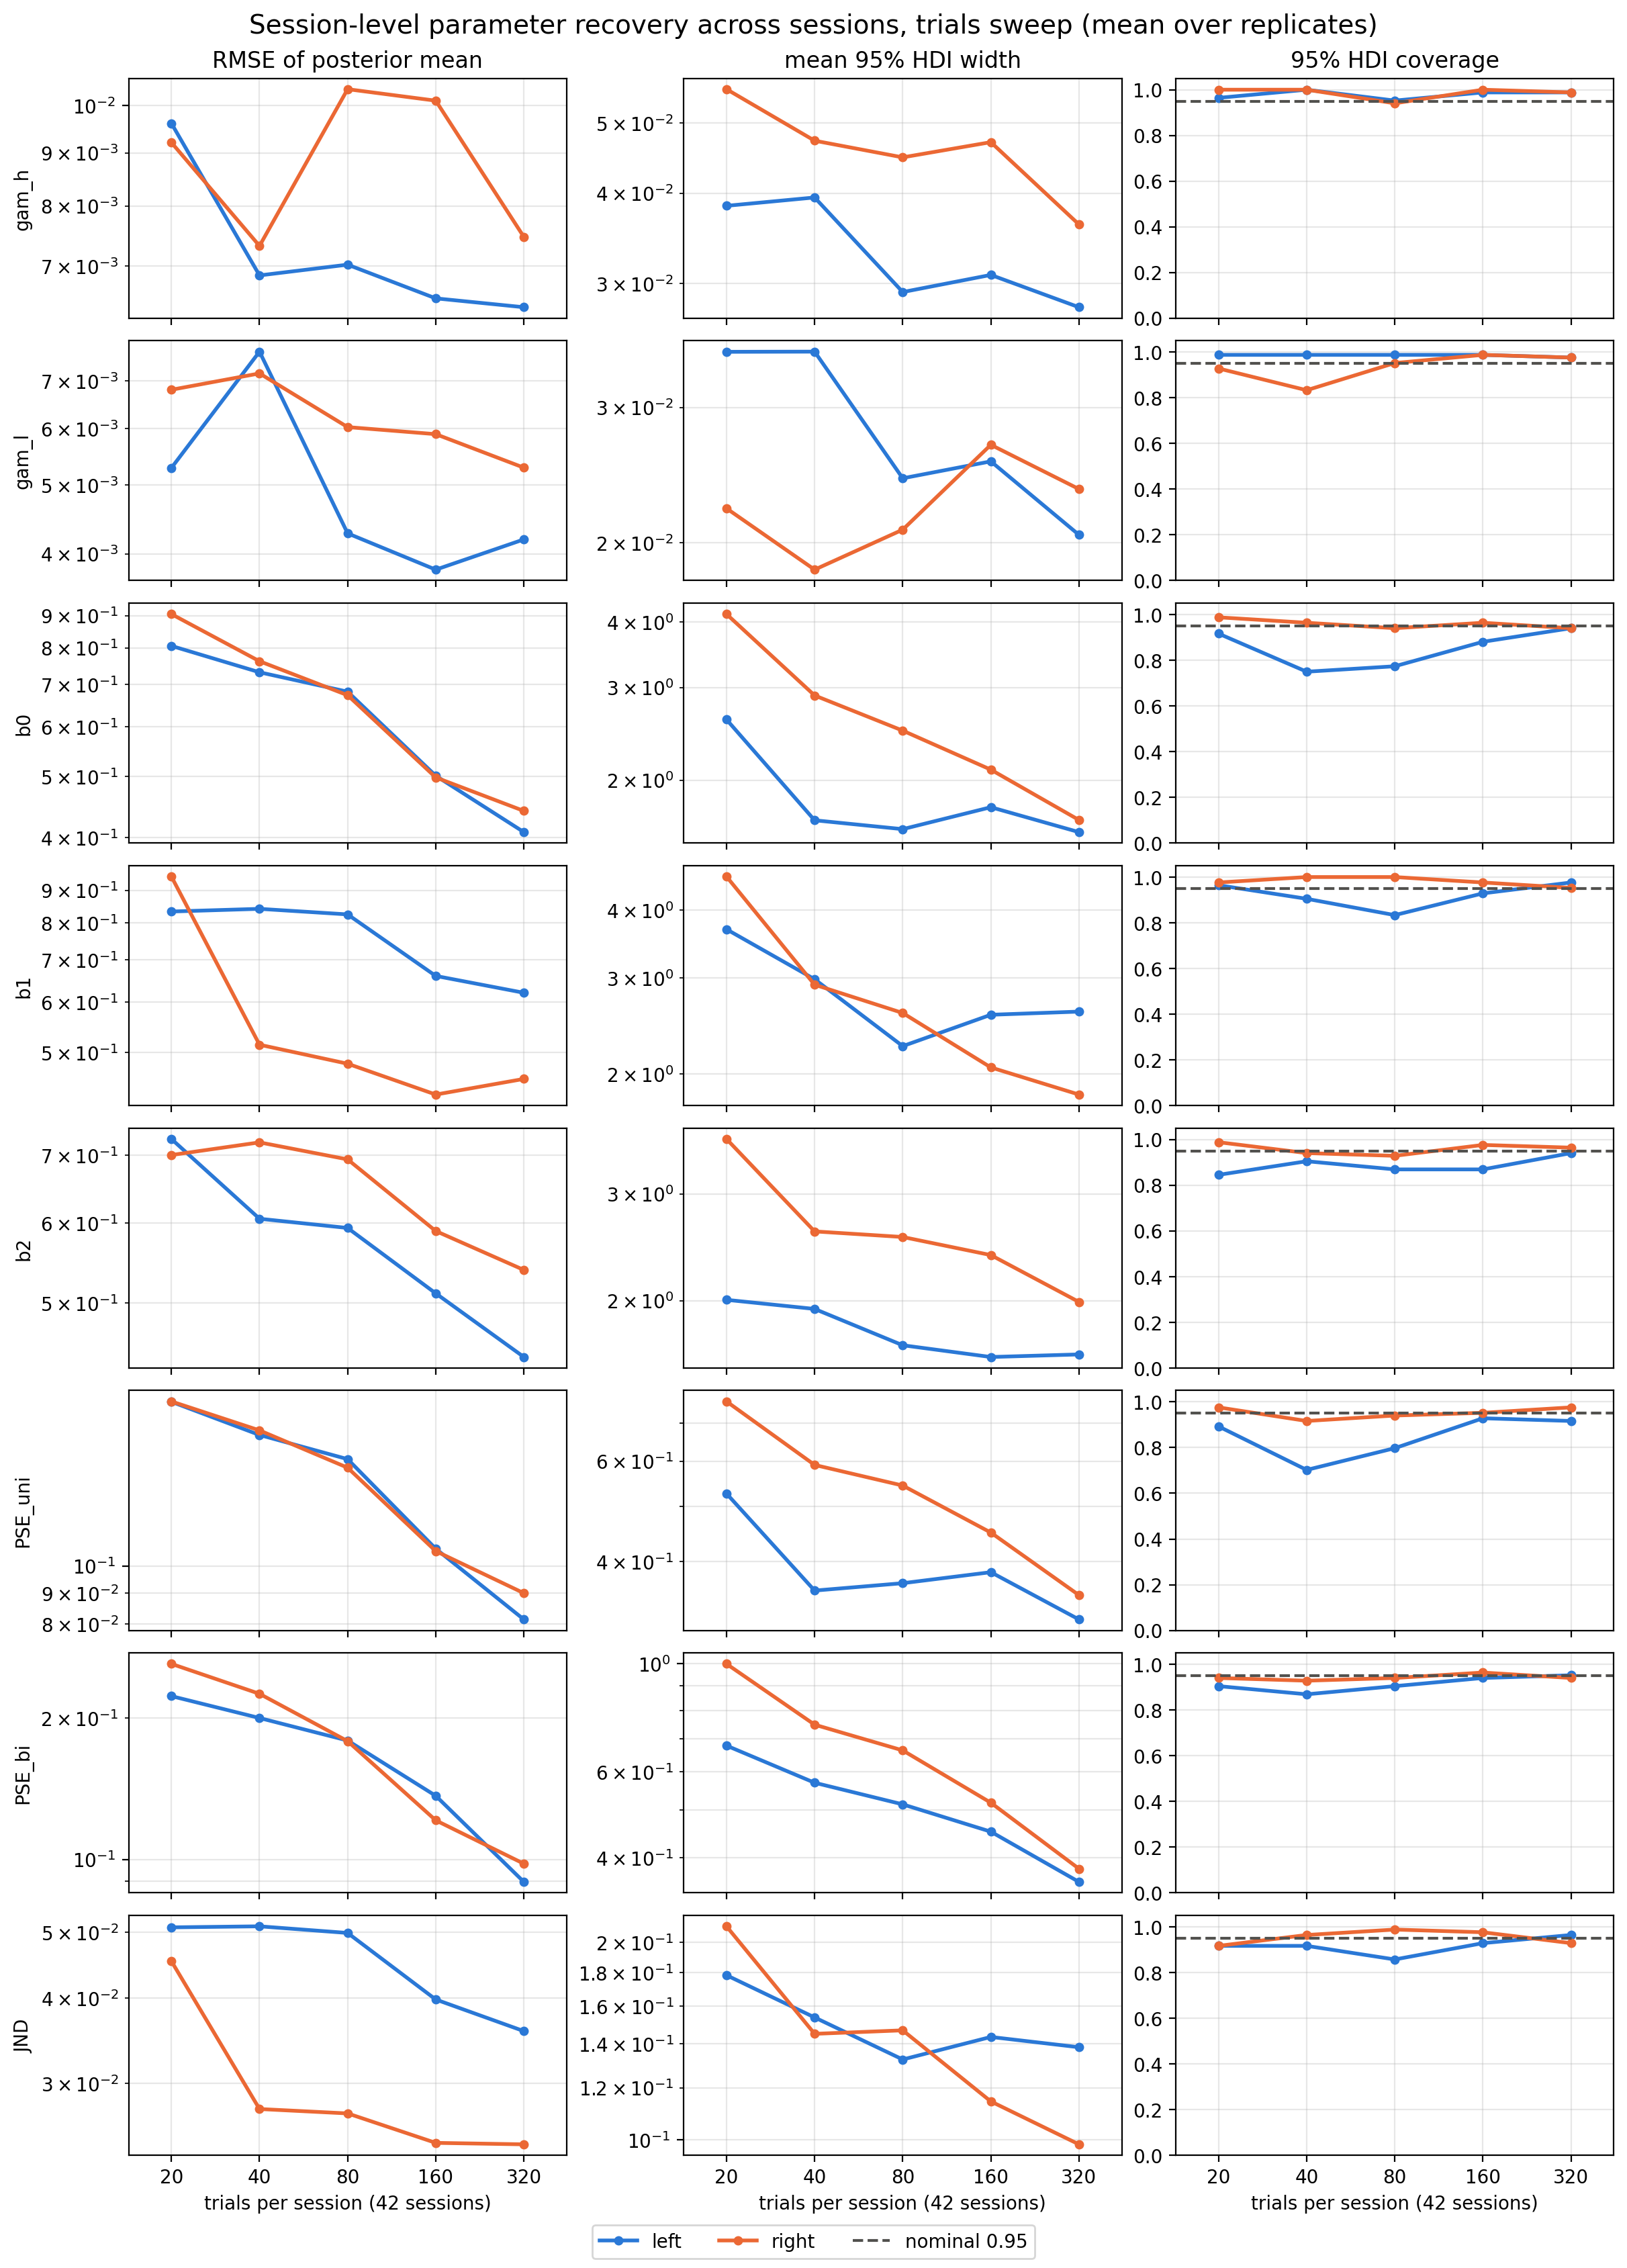
\includegraphics[width=0.92\textwidth,height=0.8\textheight,keepaspectratio]{session_params_error_width_coverage_vs_trials.png}
\caption{Session-level recovery against trials per session (42 sessions),
averaged over replicates. Left: RMSE of the posterior mean across sessions.
Middle: mean 95\% HDI width. Right: fraction of sessions whose HDI contains the
true value.}
\label{fig:session_trials}
\end{figure}

\begin{figure}[H]
\centering
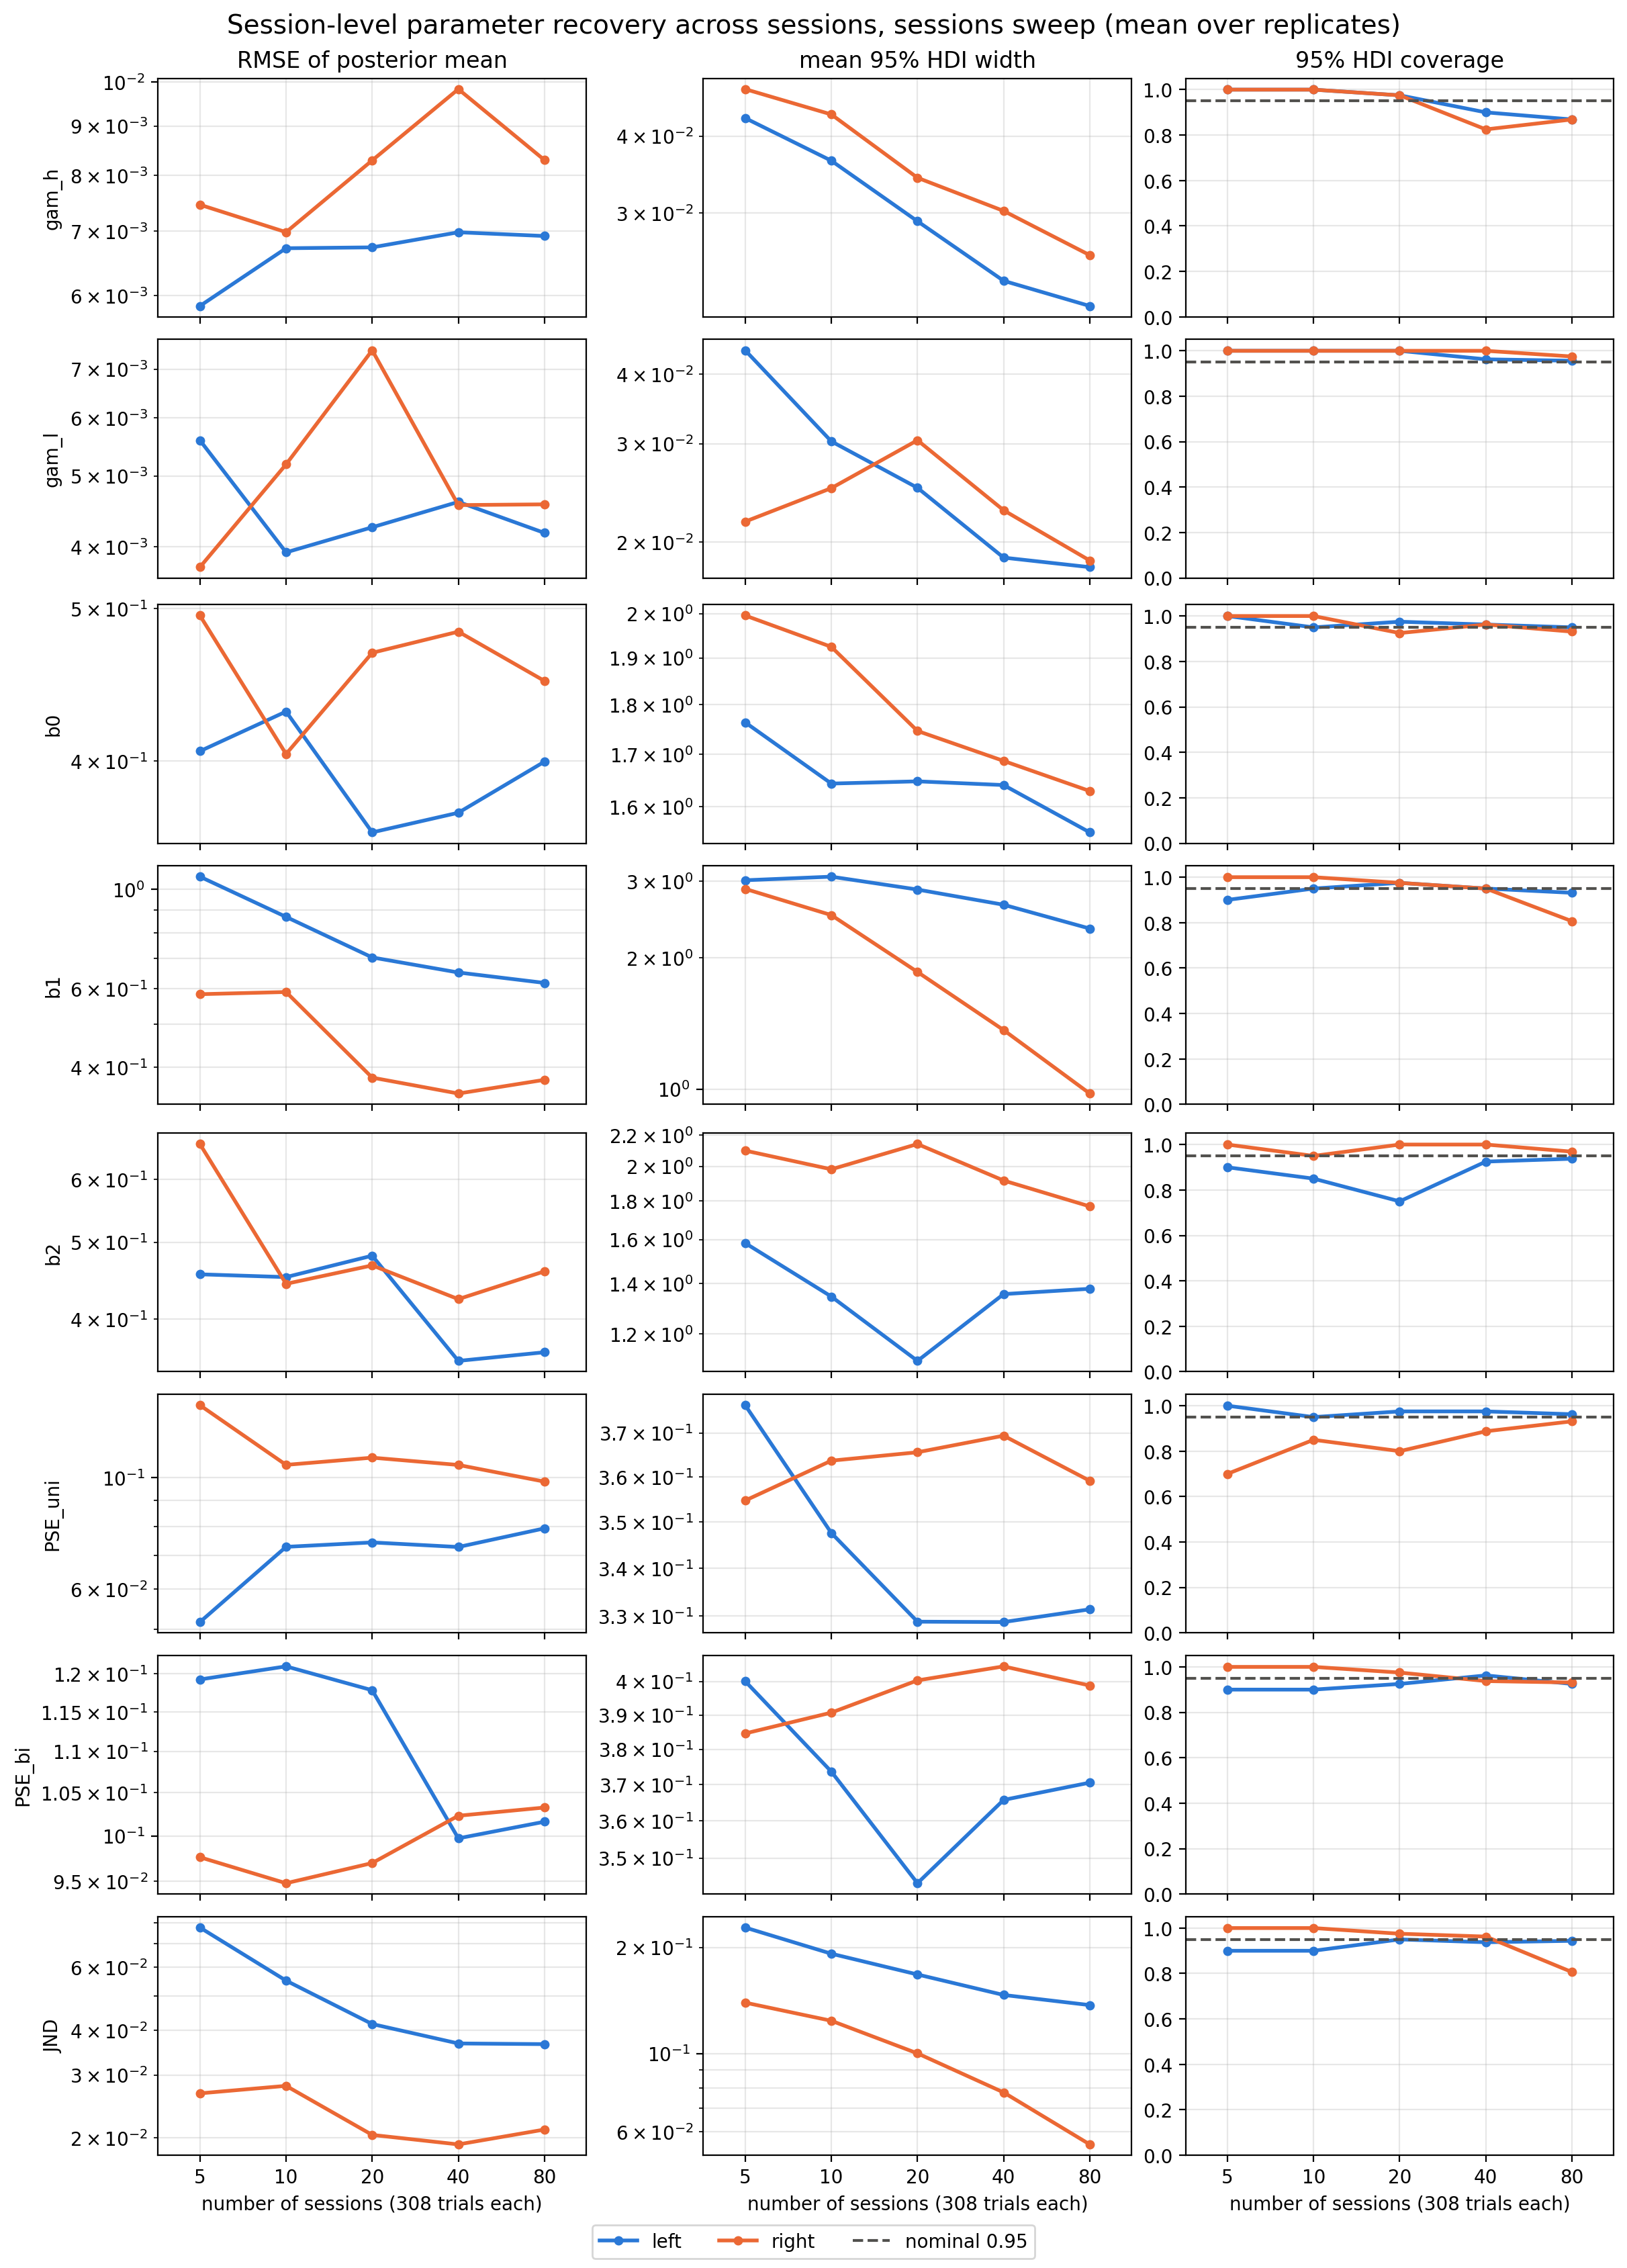
\includegraphics[width=0.92\textwidth,height=0.8\textheight,keepaspectratio]{session_params_error_width_coverage_vs_sessions.png}
\caption{As Figure~\ref{fig:session_trials}, against the number of sessions
(308 trials each).}
\label{fig:session_sessions}
\end{figure}

\begin{table}[H]
\centering
\caption{Session-level recovery at 320 trials per session (42 sessions, both
replicates): RMSE of the posterior mean / mean HDI width / coverage.}
\label{tab:session320}
\begin{tabular}{lcc}
\toprule
 & left & right \\
\midrule
PSE, unimanual & 0.083 / 0.32 / 0.92 & 0.090 / 0.35 / 0.98 \\
PSE, bimanual & 0.090 / 0.36 / 0.95 & 0.098 / 0.38 / 0.94 \\
JND & 0.036 / 0.14 / 0.96 & 0.024 / 0.10 / 0.93 \\
$\beta_0$ & 0.42 / 1.59 / 0.94 & 0.44 / 1.68 / 0.94 \\
$\beta_1$ & 0.63 / 2.60 / 0.98 & 0.46 / 1.83 / 0.95 \\
$\beta_2$ & 0.45 / 1.63 / 0.94 & 0.54 / 1.99 / 0.96 \\
$\gamma_h$ & 0.006 / 0.028 / 0.99 & 0.007 / 0.036 / 0.99 \\
$\gamma_l$ & 0.004 / 0.020 / 0.98 & 0.005 / 0.023 / 0.98 \\
\bottomrule
\end{tabular}
\end{table}

\paragraph{PSE and JND.} The per-session PSEs are recovered well in both conditions:
at 320 trials the RMSE is 0.08--0.10 standardized units, with
coverage 0.92--0.98 (Table~\ref{tab:session320}). The bimanual PSE is only slightly less
precise than the unimanual one, although it also depends on $\beta_2$. The JND
RMSE is 0.024--0.036. Error and HDI width fall steadily with trials per session
(Figure~\ref{fig:session_trials}).

\paragraph{$\beta_0$, $\beta_1$, $\beta_2$.} The individual coefficients are much less
precise than the PSEs computed from them (HDI widths 1.6--2.6 at 320 trials, against
0.32--0.38 for the PSEs): the data constrain the point where the curve crosses 0.5
better than the separate coefficients that place it there. Coverage is close to nominal at 320 trials
(0.94--0.98). At 40 and 80 trials it is lower for $\beta_0$ (0.86 at both, averaged
over hands) and the unimanual PSE (0.81 and 0.87).

\paragraph{Session-level $\beta_2$ and the distractor amplitude.}
Each session's $\beta_2$ is informed only by the shift between its unimanual and
bimanual trials at its single distractor amplitude, and that shift is $\beta_2 d_s$. A
small $d_s$ therefore leaves $\beta_2$ poorly determined
(Figure~\ref{fig:b2_sessions}, Table~\ref{tab:b2amp}): at 320 trials the HDI is
2.6 wide for sessions with a 6~$\mu$m distractor and 1.2 for 32~$\mu$m, and the
correlation between $d_s$ and HDI width is $-0.88$. Poorly determined sessions are
pulled toward the hand mean, so across sessions the posterior means vary less than
the true values: regressed on the true $\beta_2$, they have a slope of 0.43 (left)
and 0.58 (right) instead of 1. Coverage stays near nominal overall (0.94 and 0.96), so the HDIs reflect this uncertainty correctly.

\begin{figure}[H]
\centering
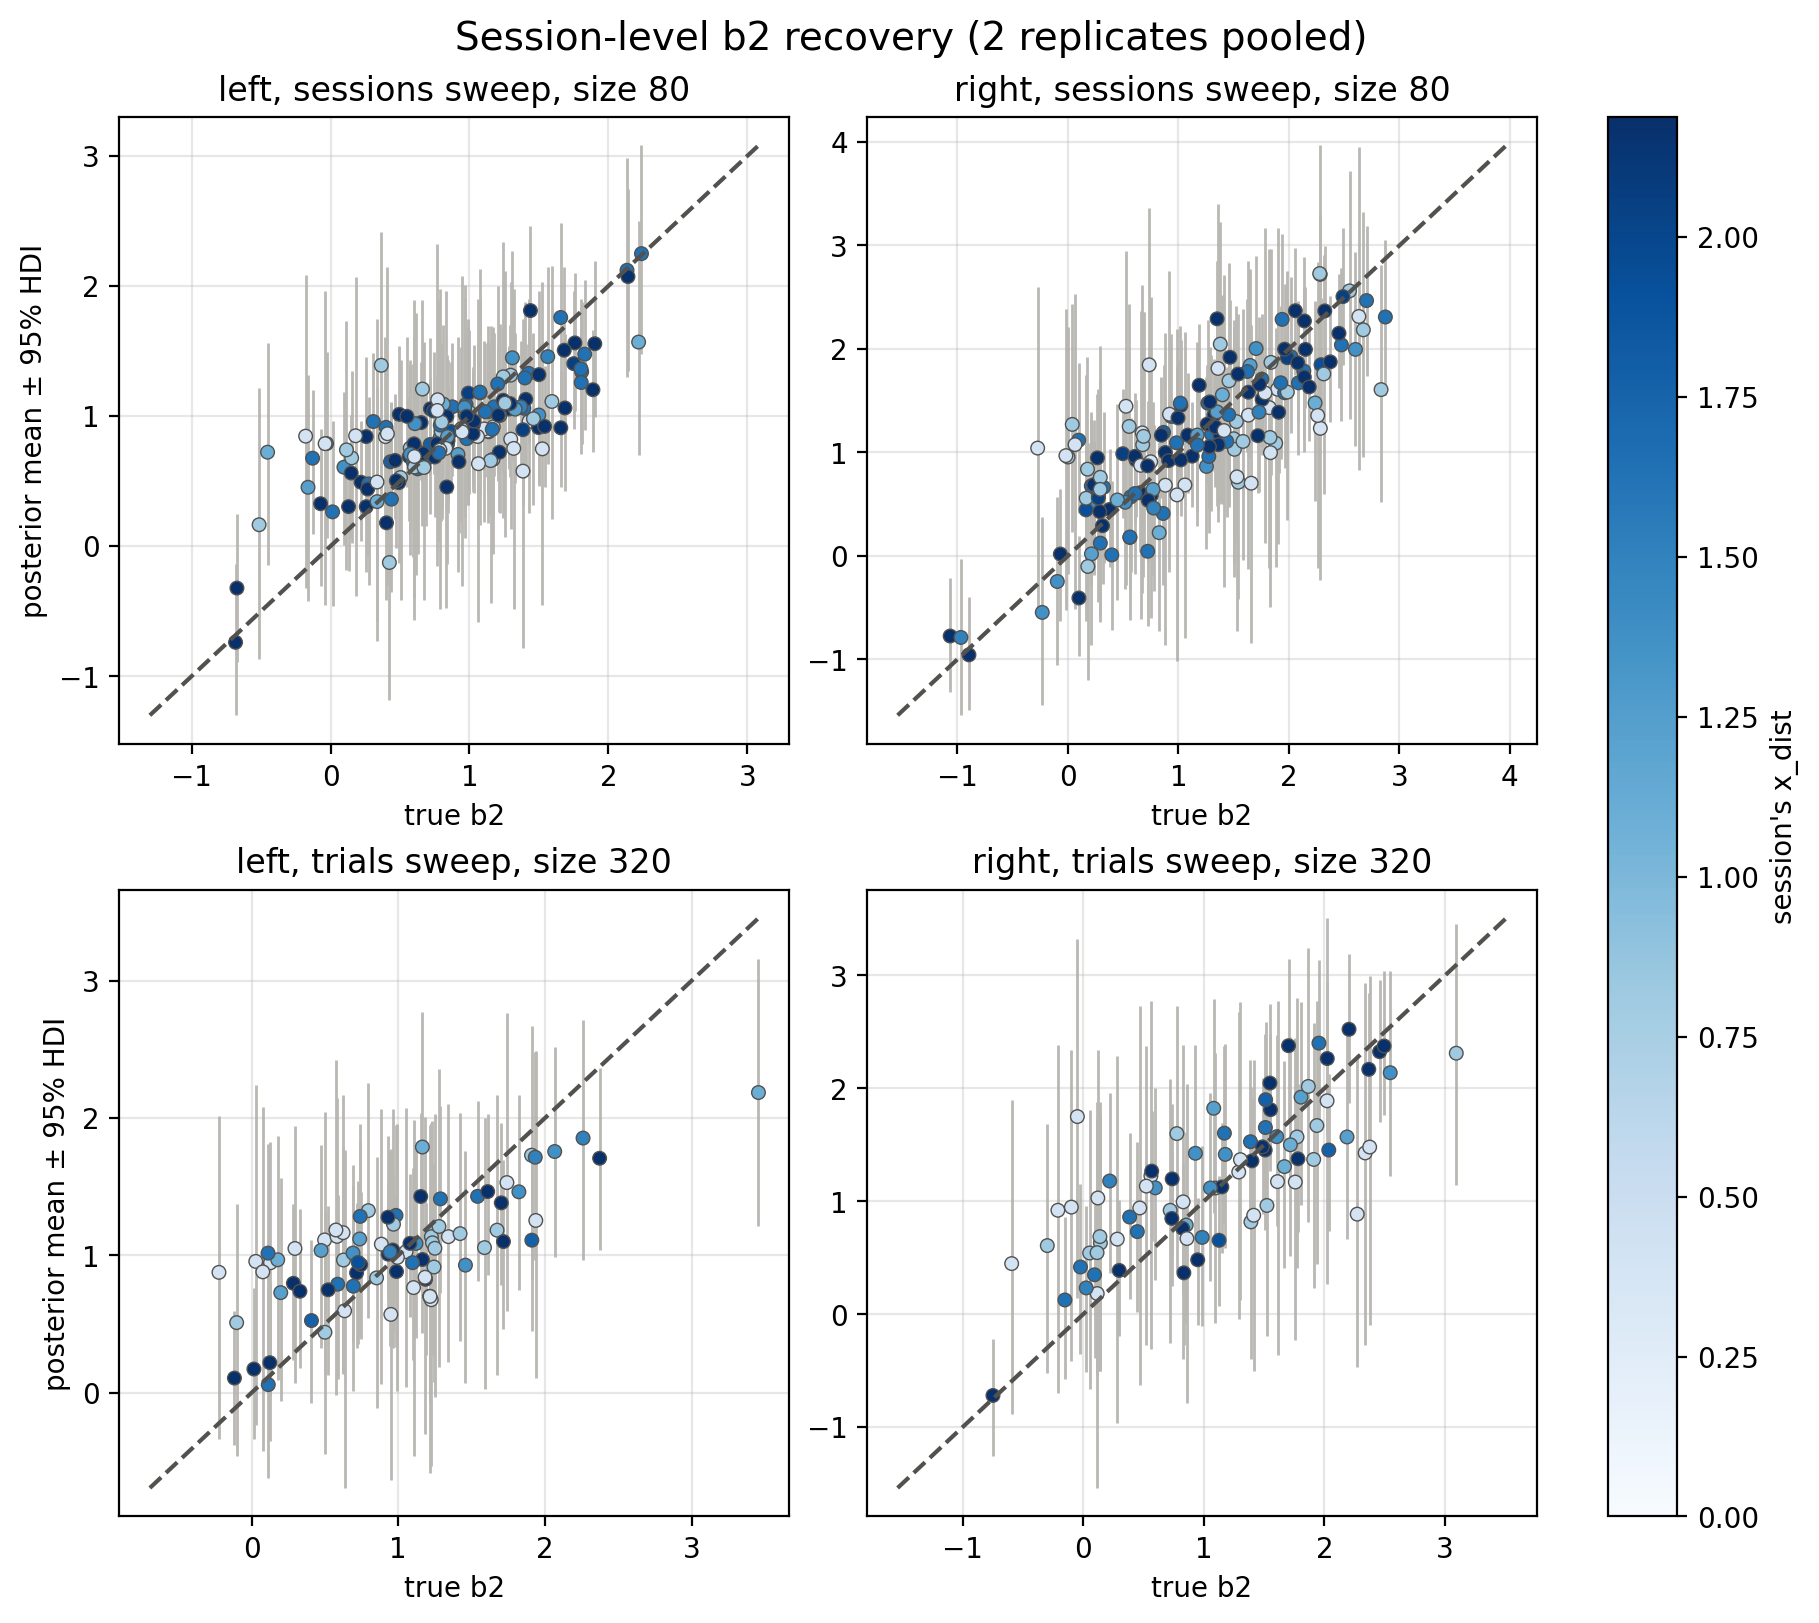
\includegraphics[width=0.85\textwidth]{session_b2_true_vs_recovered.png}
\caption{Session-level $\beta_2$: posterior mean and 95\% HDI against the true value,
colored by the session's distractor covariate $d_s$, at the largest dataset of each
sweep (both replicates pooled). The dashed line is the identity.}
\label{fig:b2_sessions}
\end{figure}

\begin{table}[H]
\centering
\caption{Session-level $\beta_2$ by distractor amplitude at 320 trials per session
(both hands and replicates pooled; $n$ = number of session estimates).}
\label{tab:b2amp}
\begin{tabular}{rcccc}
\toprule
amplitude ($\mu$m) & $n$ & RMSE & mean HDI width & coverage \\
\midrule
6  & 42 & 0.69 & 2.58 & 0.98 \\
12 & 30 & 0.44 & 2.08 & 1.00 \\
16 & 6  & 0.68 & 1.85 & 0.83 \\
18 & 6  & 0.53 & 1.69 & 1.00 \\
20 & 12 & 0.37 & 1.62 & 1.00 \\
22 & 6  & 0.46 & 1.56 & 0.83 \\
24 & 18 & 0.36 & 1.43 & 0.94 \\
26 & 4  & 0.54 & 1.33 & 0.75 \\
28 & 2  & 0.37 & 1.17 & 1.00 \\
32 & 42 & 0.32 & 1.19 & 0.93 \\
\bottomrule
\end{tabular}
\end{table}

\paragraph{Lapse rates $\gamma_h$ and $\gamma_l$.} At 320 trials the session lapse
rates have RMSE 0.004--0.007 and coverage 0.98--0.99. In the sessions sweep the coverage
of $\gamma_h$ is lower at 40 and 80 sessions (0.86 and 0.87, averaged over hands). With
$\sigma_{\gamma_h}$ not identified, the session values are pulled strongly toward the
hand's typical value, so a miss in that value likely carries over to every session of
the hand; at 40 sessions, for example, the right hand's $\mu_{\gamma_h}$ averages $-2.60$
against a true $-2.41$.

\subsection{Posterior densities}

The following plots show the same fits as full posterior densities, darker for
larger datasets. They confirm the points above: the means and the sds of the logistic
coefficients concentrate around the truth as data grow, while the posteriors of
$\sigma_{\gamma_h}$ and $\sigma_{\gamma_l}$ barely change.

\begin{figure}[H]
    \centering
    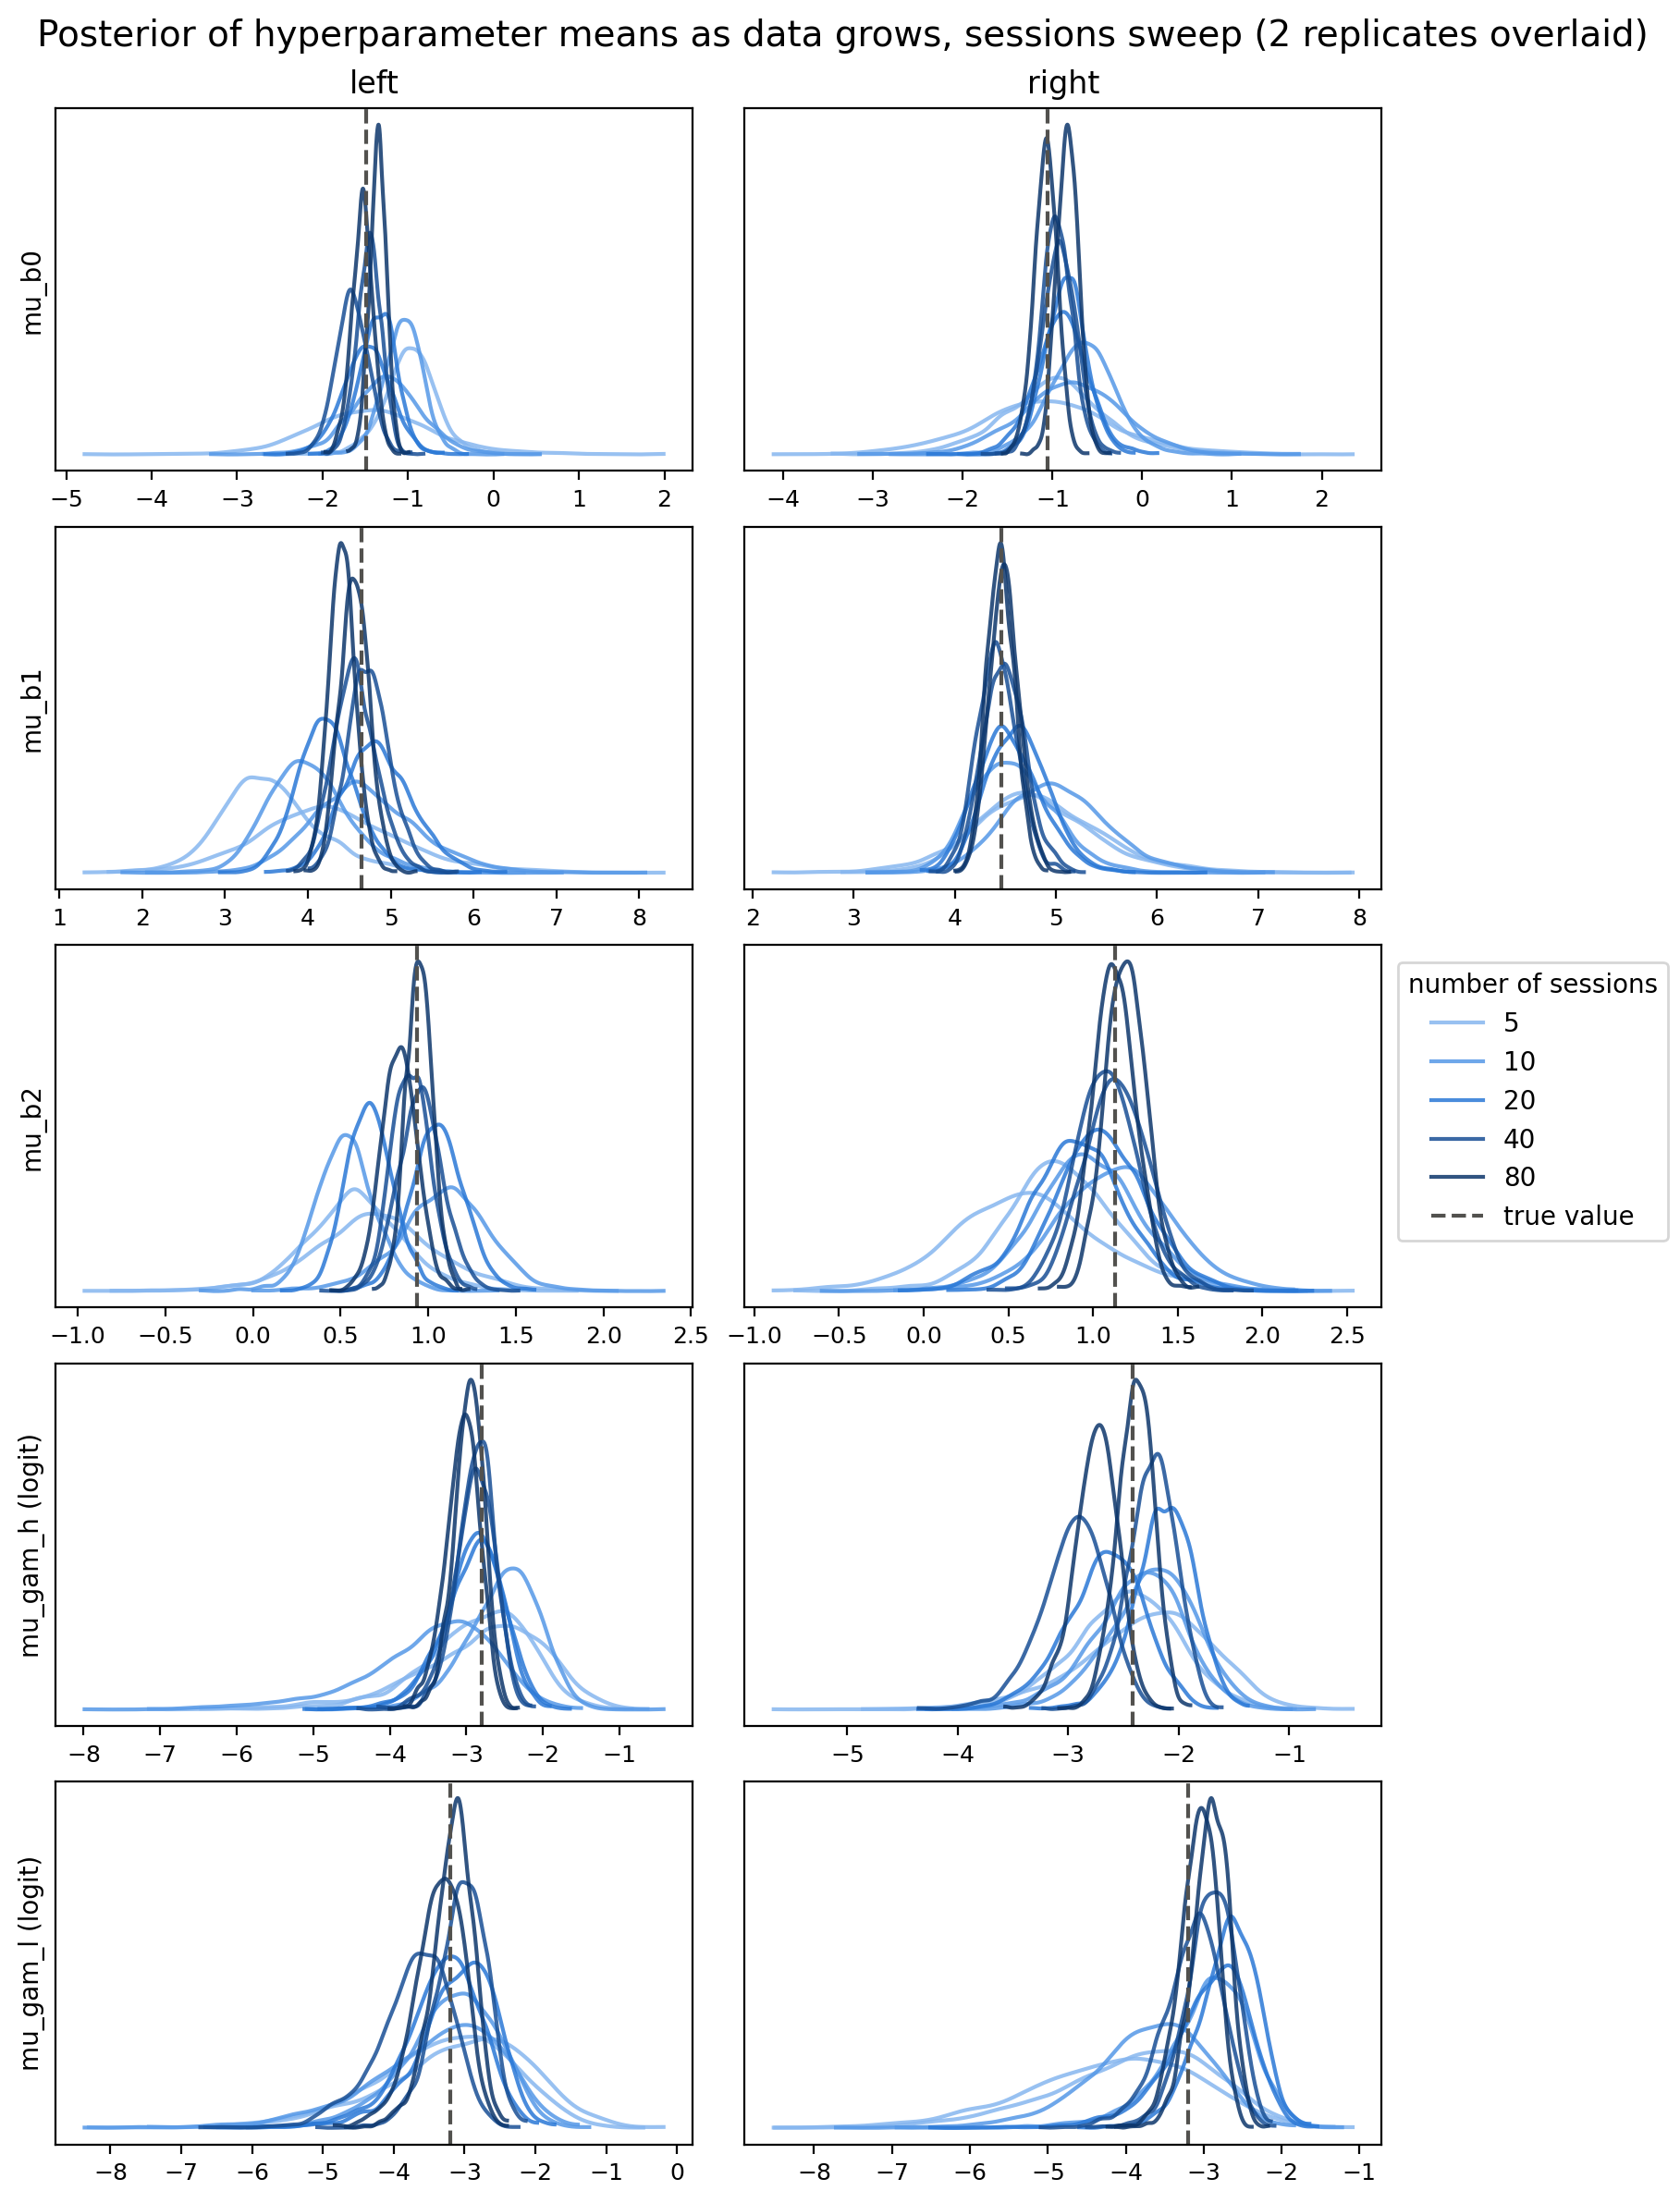
\includegraphics[width=0.9\linewidth]{hyper_means_density_vs_sessions.png}
    \caption{Posteriors of mean hyperparameters as sessions vary}
\end{figure}

\begin{figure}[H]
    \centering
    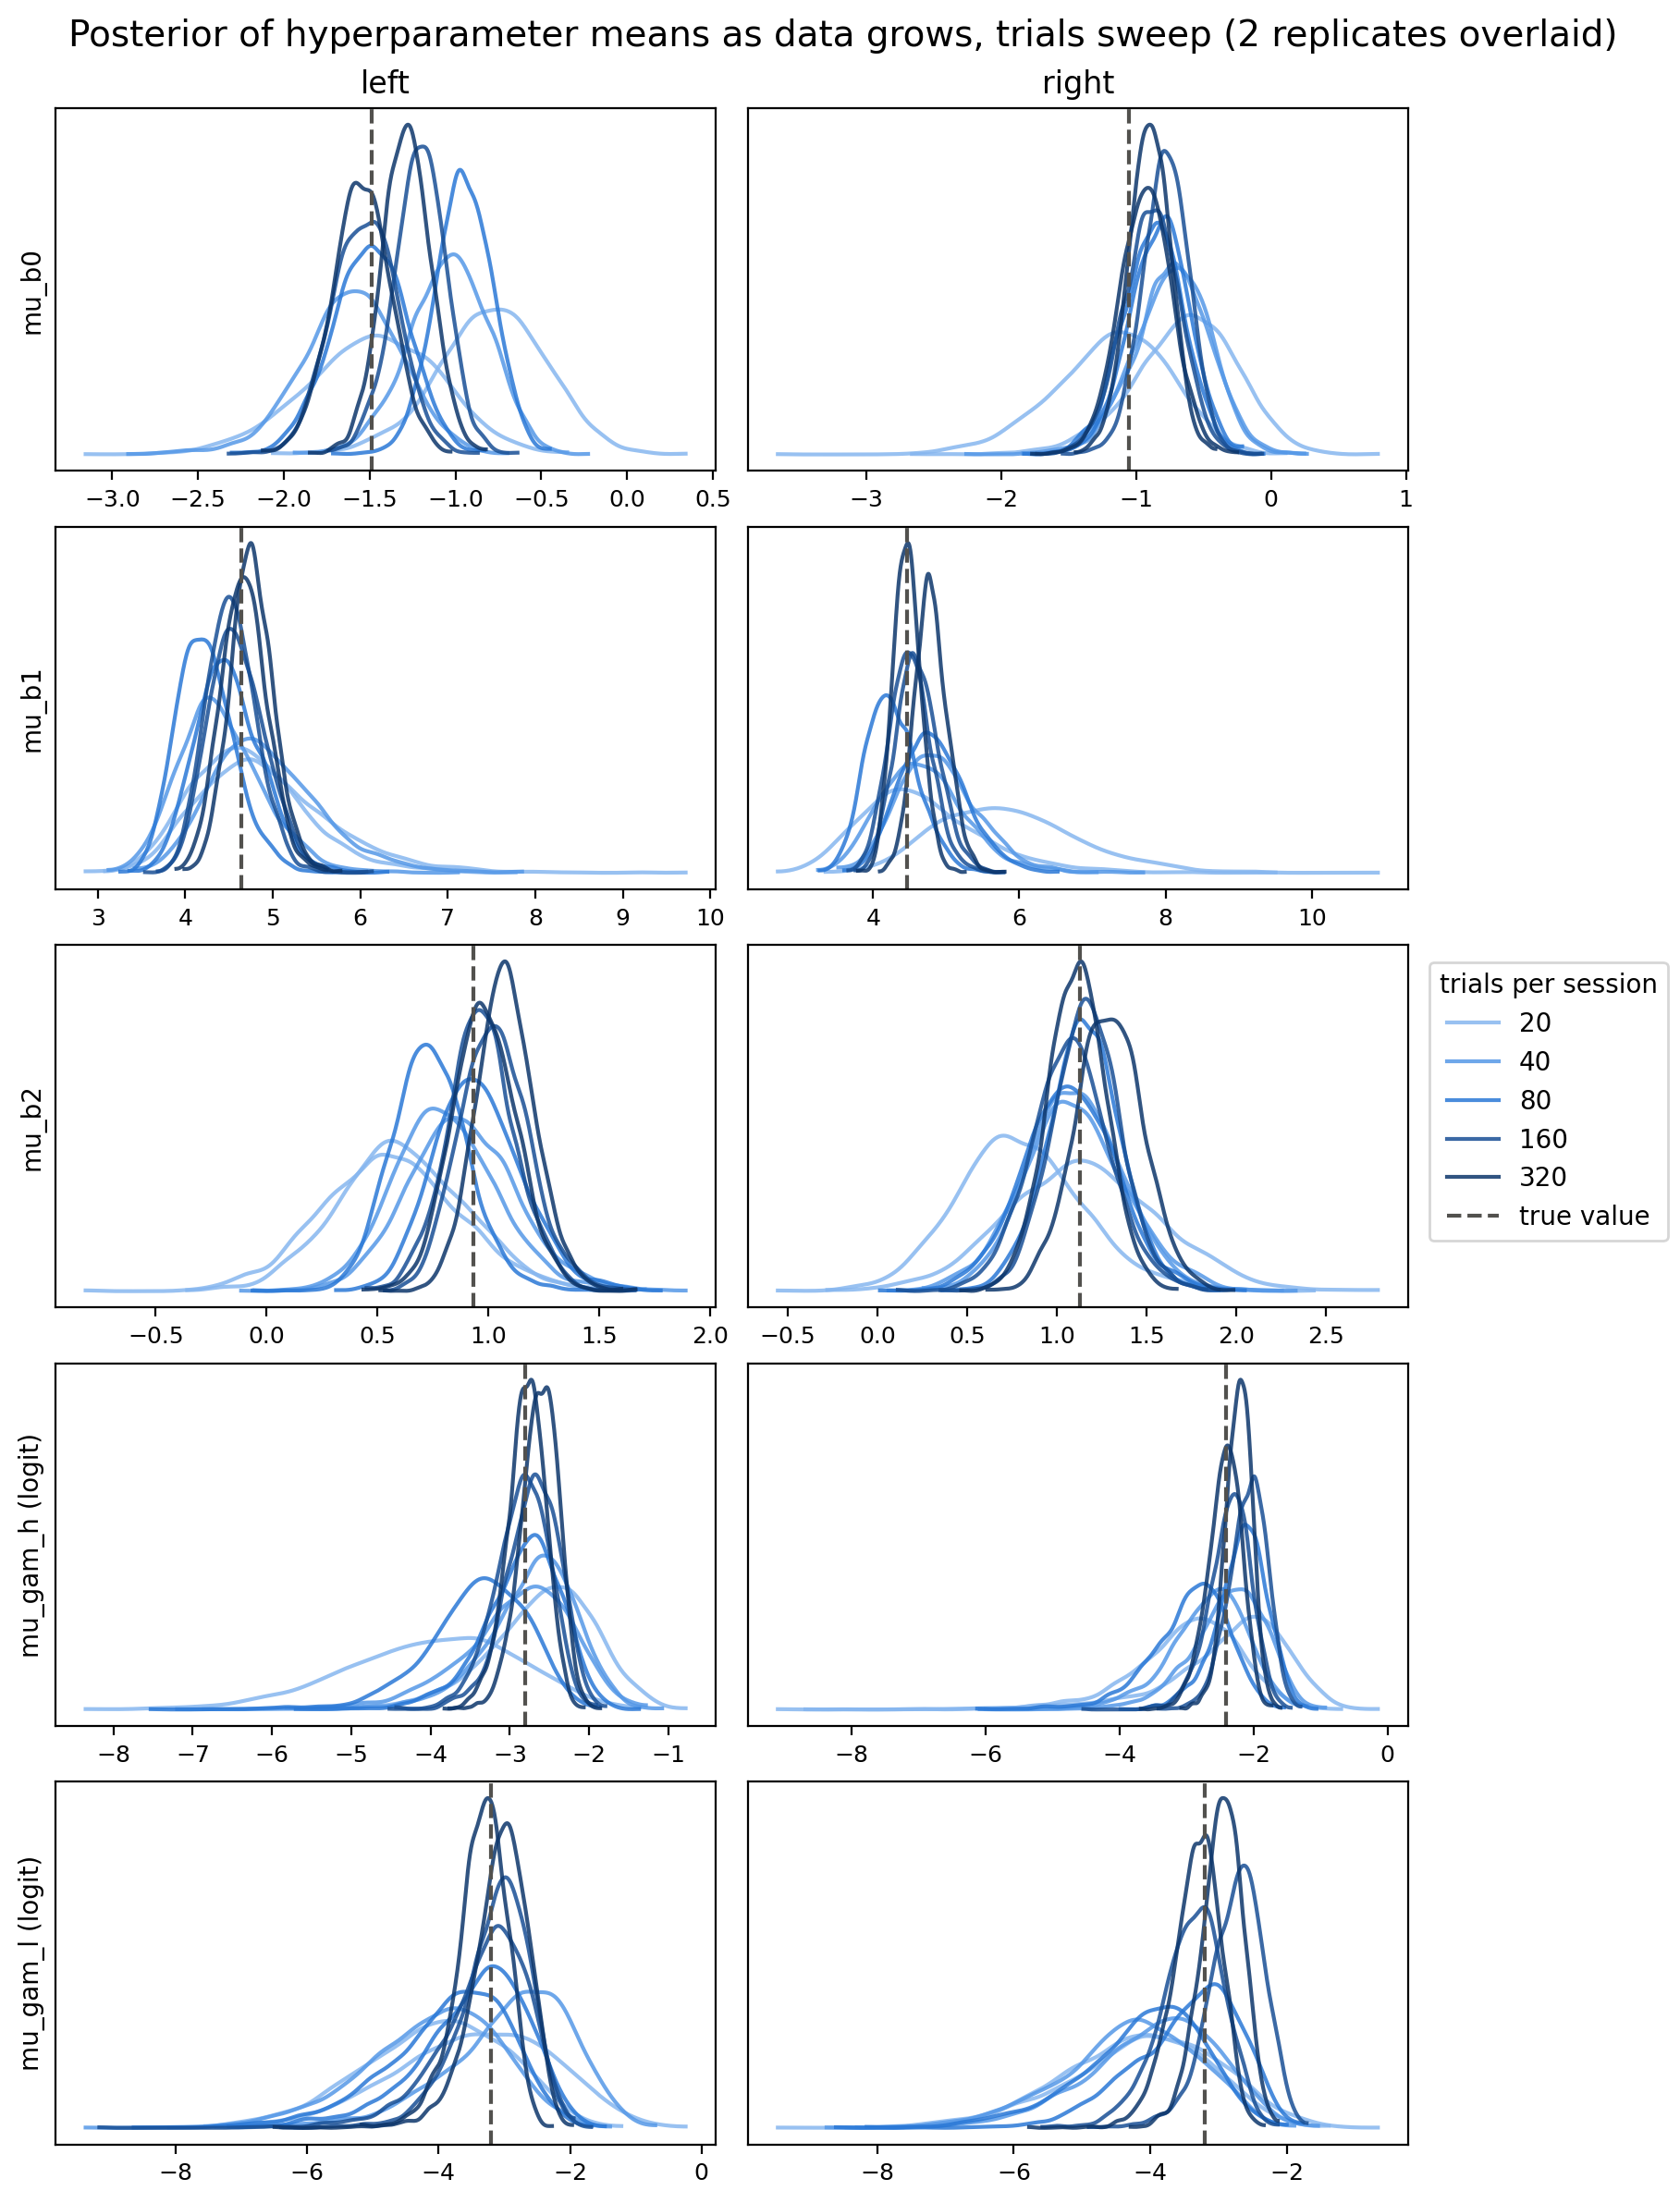
\includegraphics[width=0.9\linewidth]{hyper_means_density_vs_trials.png}
    \caption{Posteriors of mean hyperparameters as trials vary}
\end{figure}

\begin{figure}[H]
    \centering
    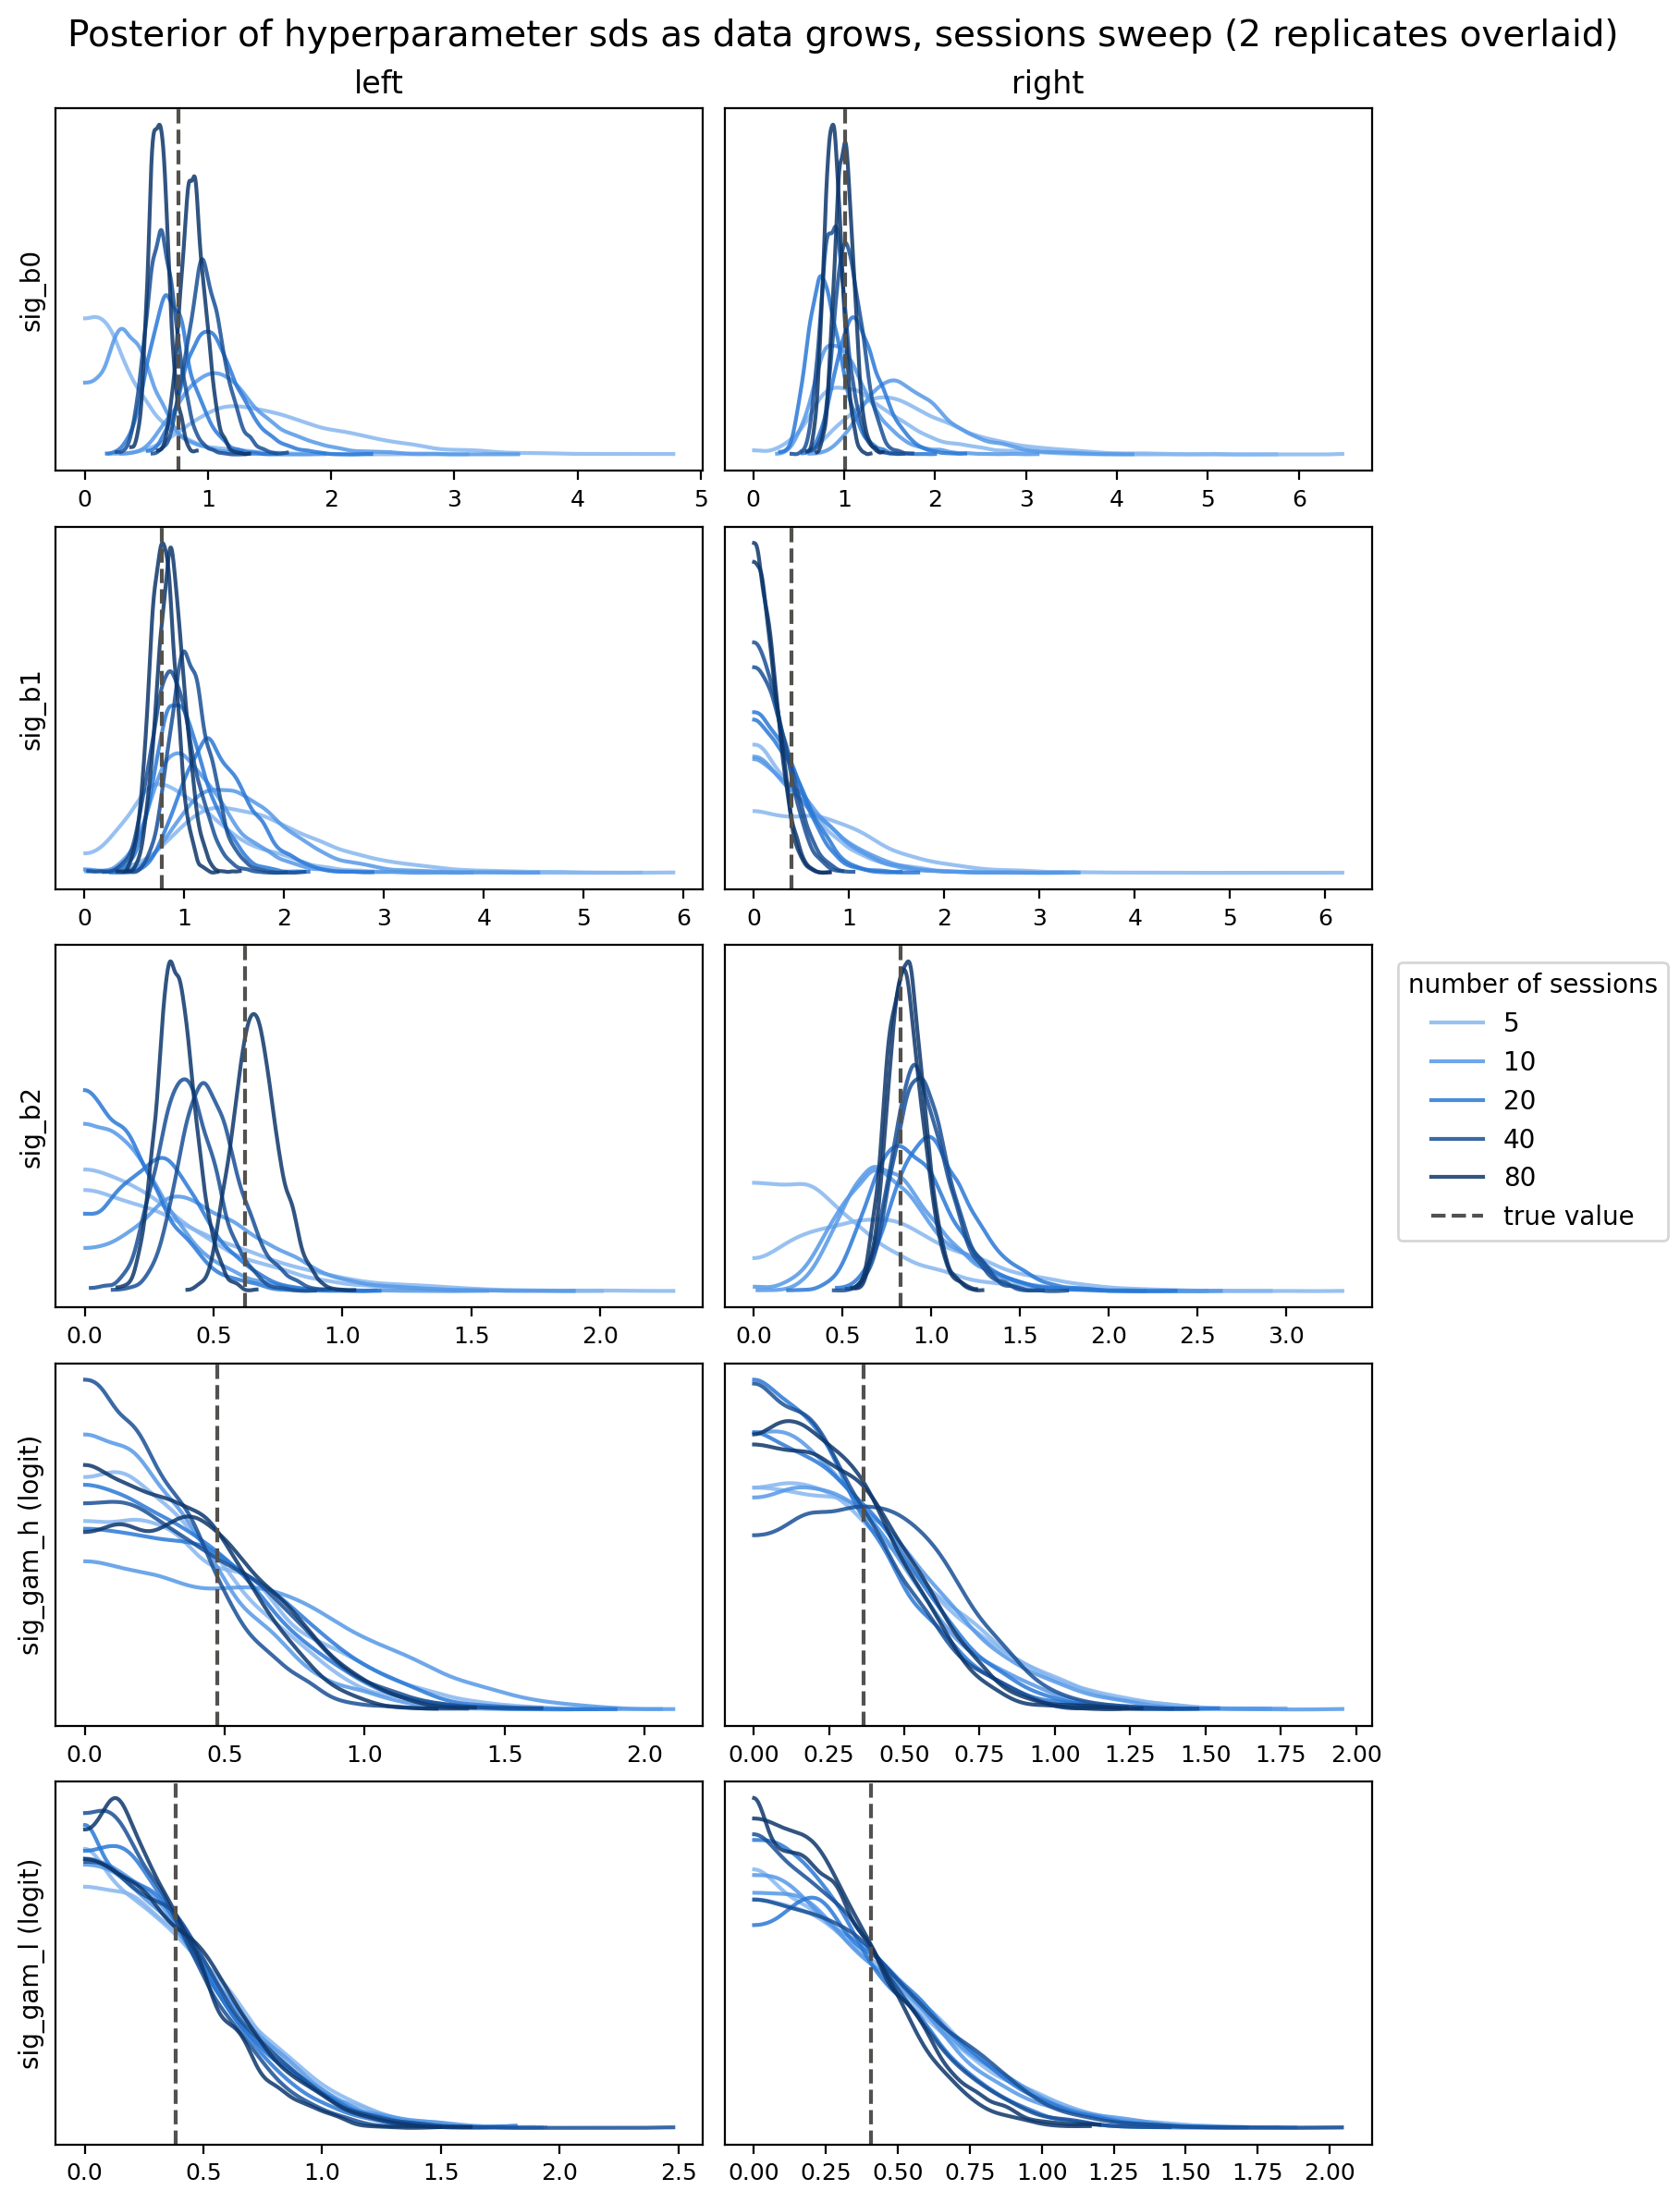
\includegraphics[width=0.9\linewidth]{hyper_sds_density_vs_sessions.png}
    \caption{Posteriors of sd hyperparameters as sessions vary}
\end{figure}

\begin{figure}[H]
    \centering
    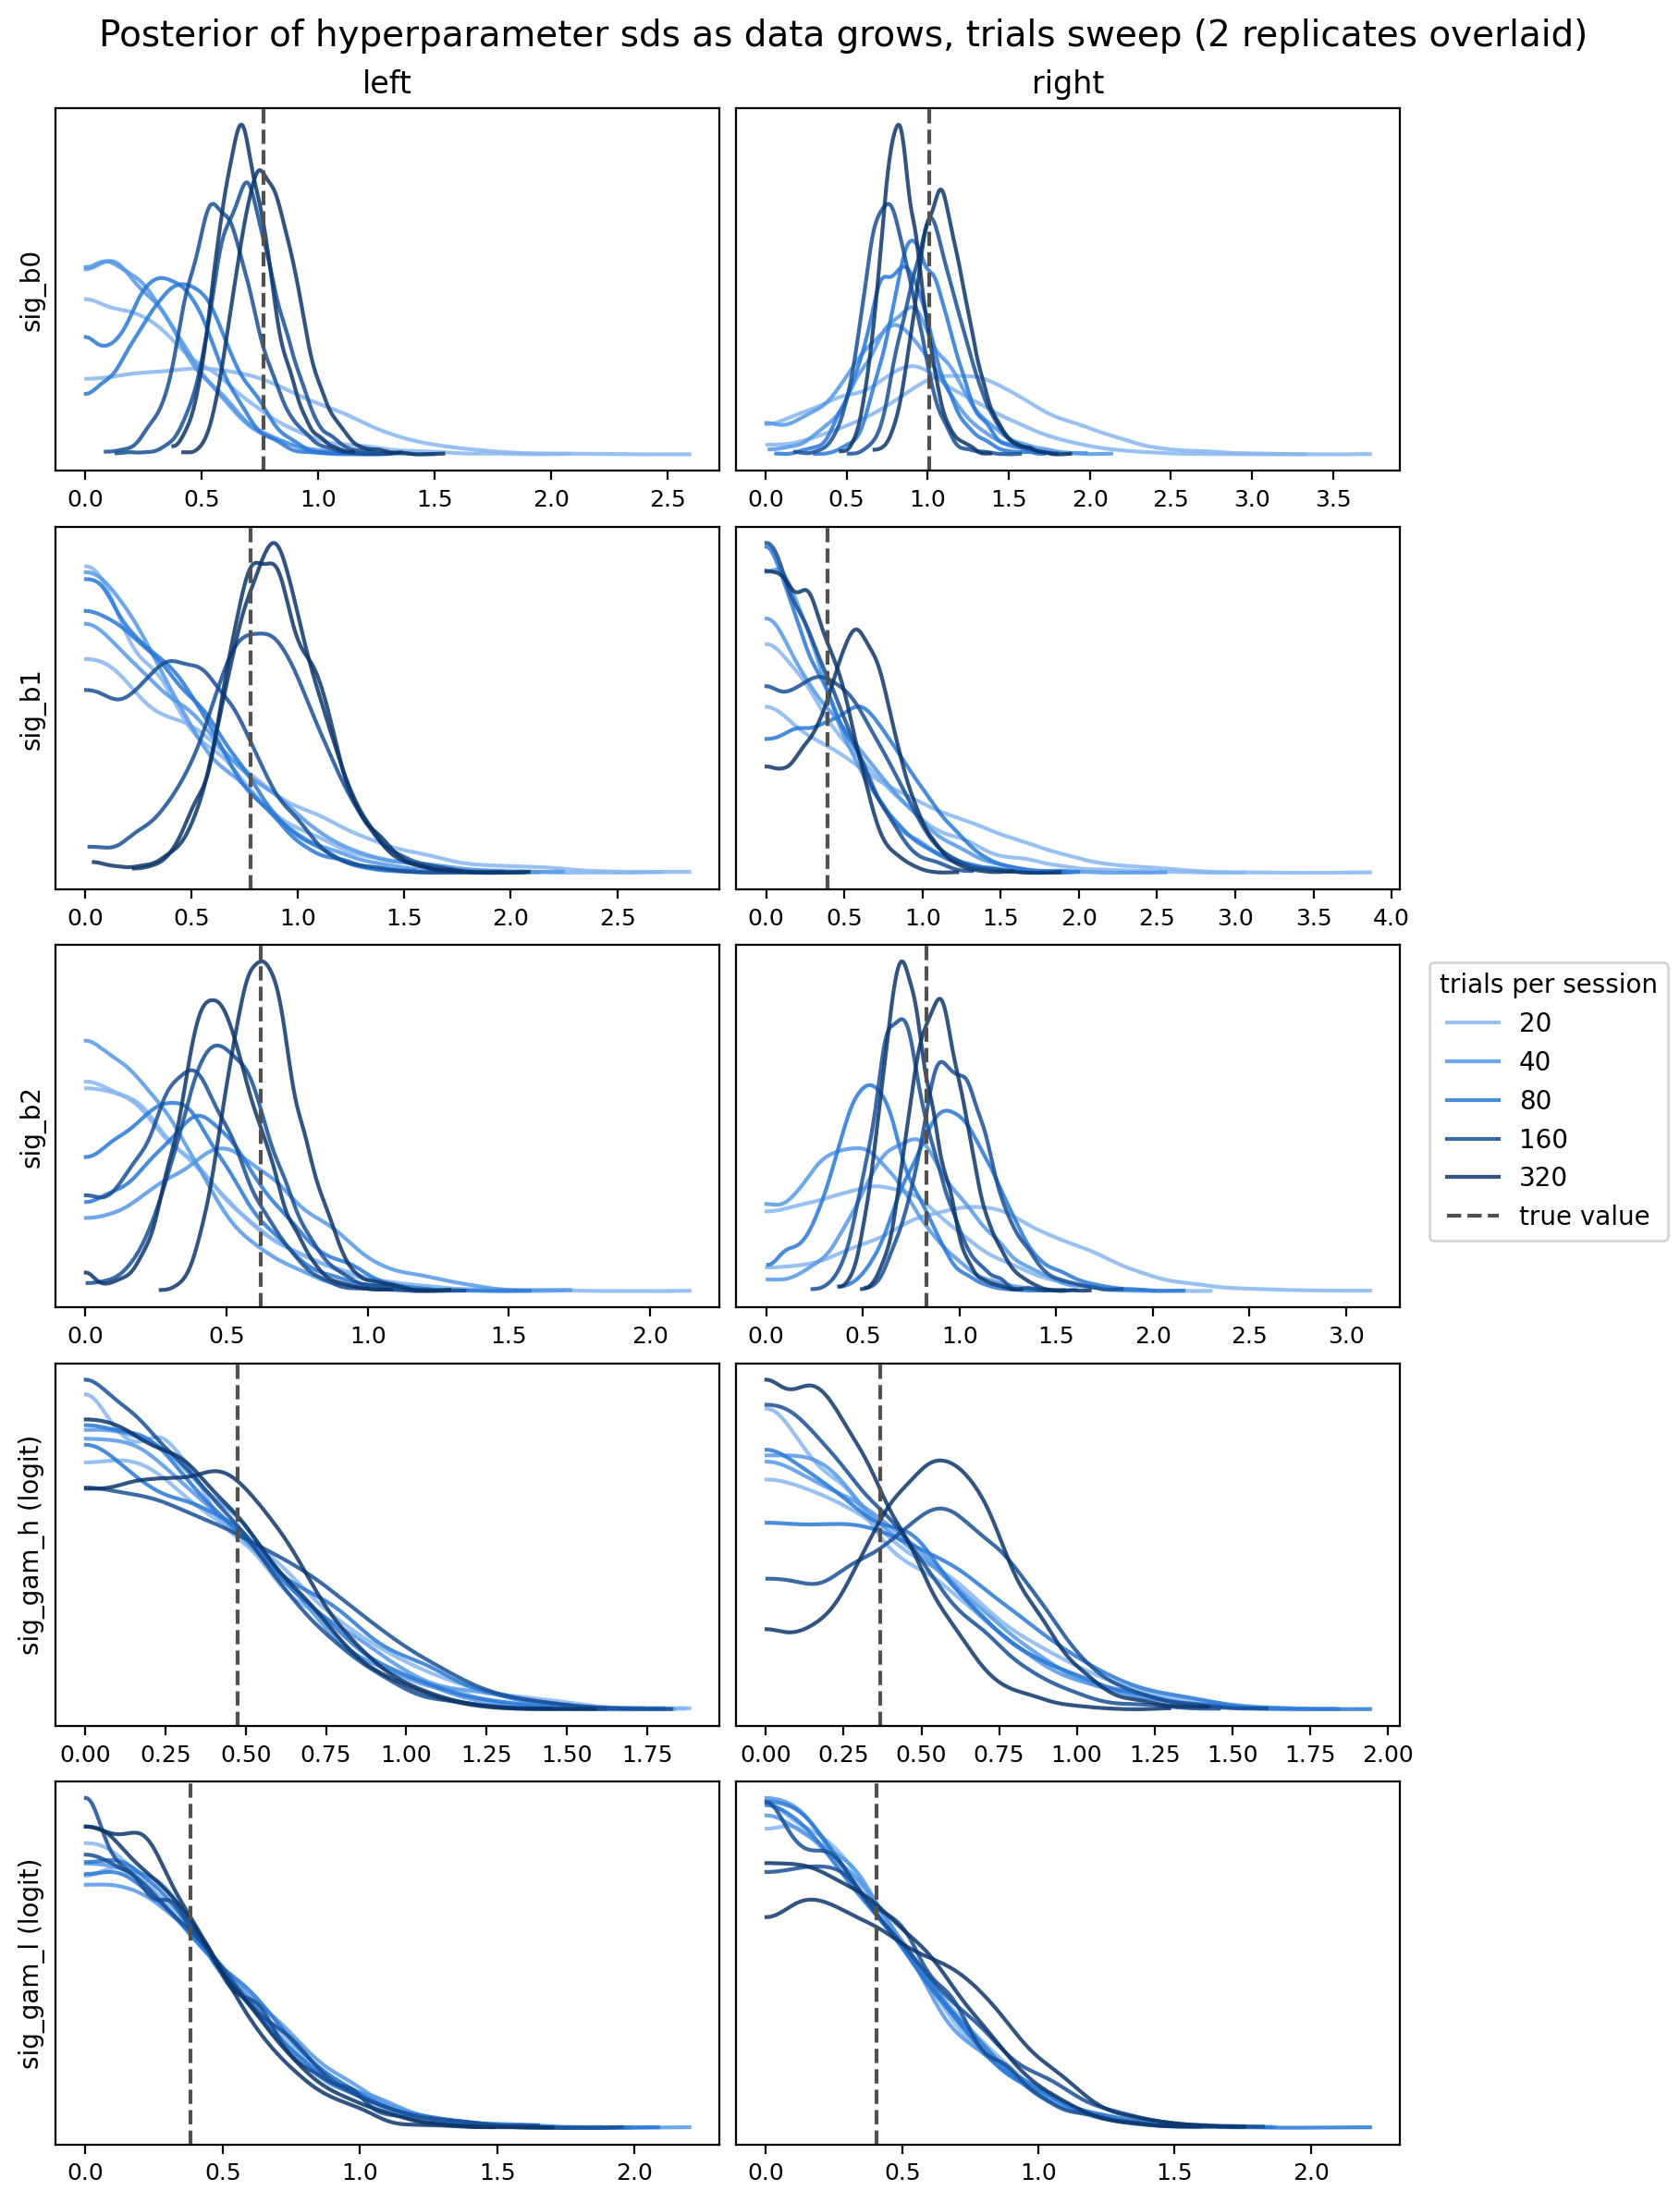
\includegraphics[width=0.9\linewidth]{hyper_sds_density_vs_trials.png}
    \caption{Posteriors of sd hyperparameters as trials vary}
\end{figure}

\begin{figure}[H]
\centering
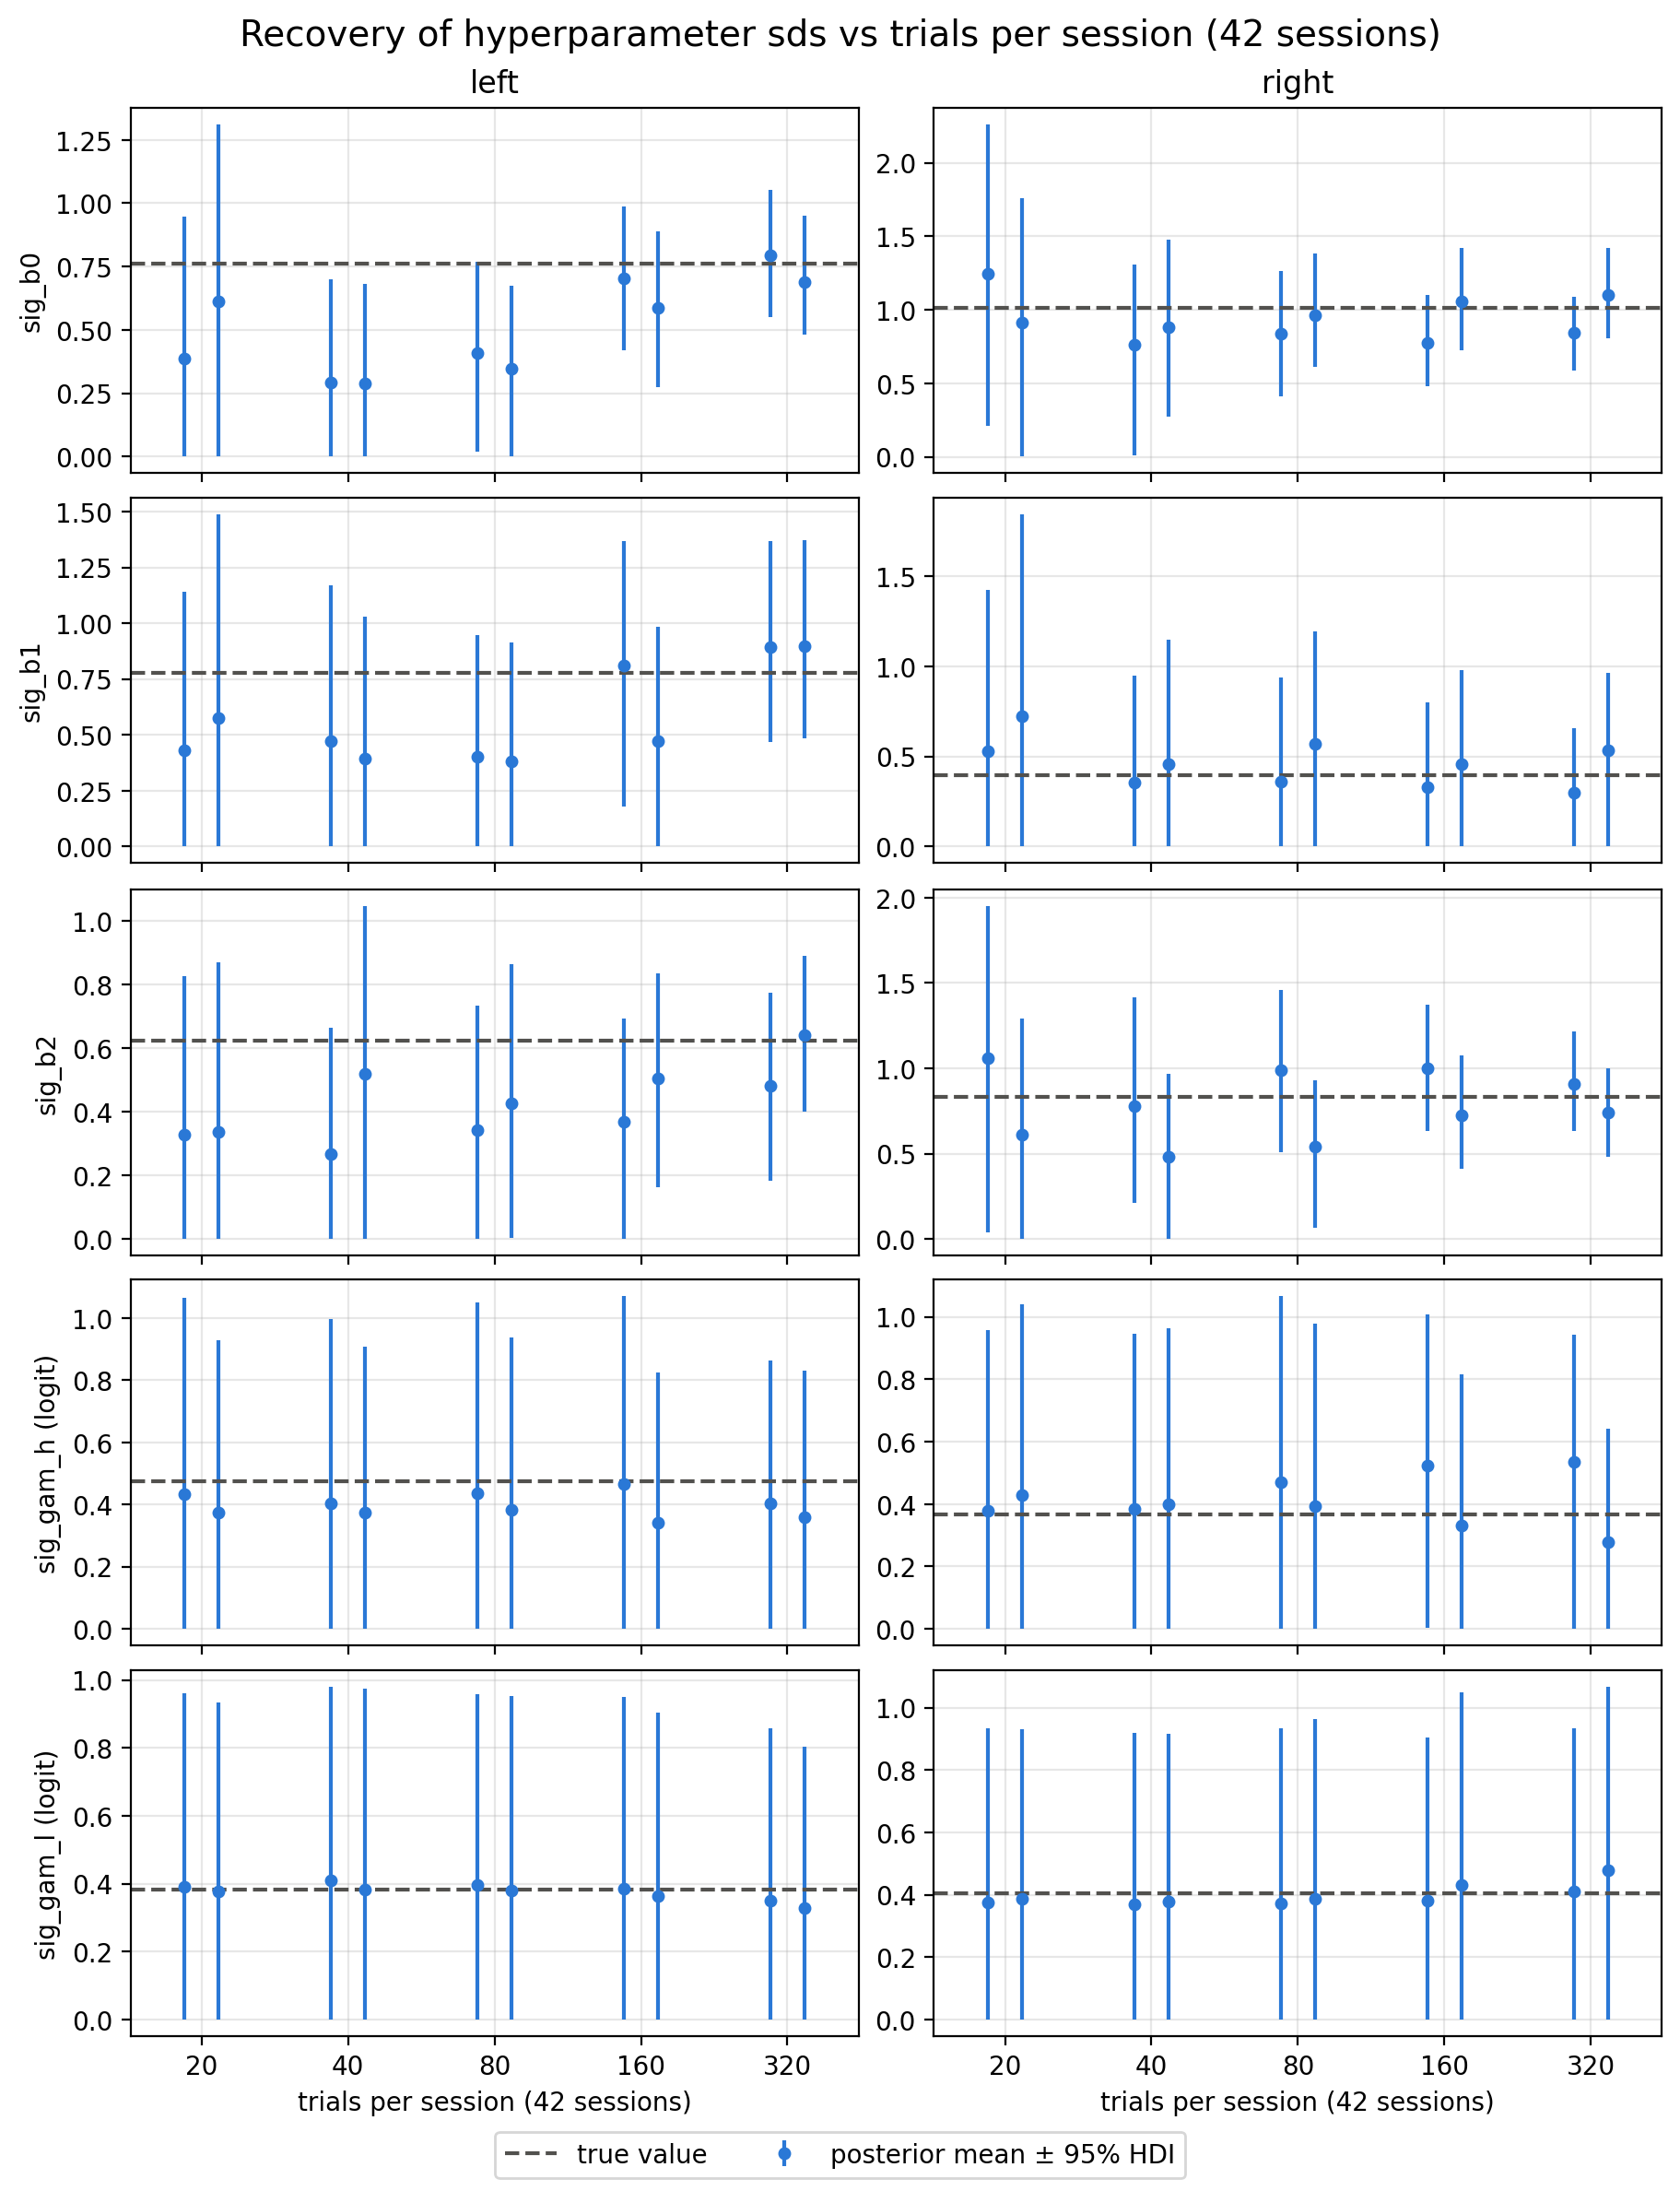
\includegraphics[width=0.9\textwidth]{hyper_sds_recovery_vs_trials.png}
\caption{Posterior mean and 95\% HDI of the between-session sds against trials per
session (42 sessions).}
\end{figure}

\subsection{Conclusions for the real data}

At the size of the real dataset (42 sessions of about 308 trials), if the data follow
Model C:

\begin{itemize}
  \item \textbf{Reliable:} per-session PSEs in both conditions and JNDs; all five
        hand-level means, including the distractor effect $\mu_{\beta_2}$, whose HDI
        (0.47--0.73 wide at 40 sessions) is narrow enough to tell an effect of the
        size simulated here from 0; the between-session sds of $\beta_0$, $\beta_1$
        and $\beta_2$, with the caveats above.
  \item \textbf{Weakly determined:} the individual session coefficients, especially
        $\beta_2$ for sessions with small distractors, which are pulled toward the hand
        mean. Session-level $\beta_2$ values should not be compared across sessions
        without their HDIs.
  \item \textbf{Not identified:} $\sigma_{\gamma_h}$ and $\sigma_{\gamma_l}$. Their
        posteriors largely reflect the priors and should not be interpreted.
  \item The sampler had no real difficulties: 2 divergences in 20 fits, both in the
        smallest datasets.
\end{itemize}

\paragraph{What this study does not test.} The synthetic data follow Model C
exactly. In particular, the unimanual and bimanual trials of a session share their
lapse rates, and the distractor effect is linear in amplitude. Model B's fit to the
real data suggests that $\gamma_h$ is higher on bimanual than on unimanual trials, and
the synthetic data built from that fit already show more low-stimulus lapses on
unimanual trials than the real data do (the comparison printed by
\code{DataProcessing\_C.py}). How Model C behaves when these assumptions
fail is a question for a fit to the real data and a model comparison with Model B.

\paragraph{Possible follow-ups.}
\begin{enumerate}
  \item Fit Model C to the real data and compare it with Model B by LOO, as was done
        for Models A and B.
  \item Consider lapse rates per hand and condition (unimanual, bimanual), keeping
        $\beta_2$ for the distractor's effect on the curve's position.
  \item Consider removing the session-level variation of the lapse rates, since
        $\sigma_{\gamma_h}$ and $\sigma_{\gamma_l}$ are not identified (as in Model B).
\end{enumerate}

\end{document}
